\documentclass{exam}
\usepackage[utf8]{inputenc}
\usepackage{amsmath}
\usepackage[shortlabels]{enumitem}
\usepackage{tikz}
\usepackage{subcaption}
\usepackage{multicol}
\graphicspath{{./graphs}}
\newcommand{\chinese}[1]{\begin{CJK}{UTF8}{gbsn}#1\end{CJK}}
\newcommand{\plane}[1][5]{
    \draw[very thin,color=gray] (-{#1},-{#1}) grid ({#1},{#1});
    \draw[thick,<->] (-{#1},0) -- ({#1},0) node[anchor=north west] {$x$};
    \draw[thick,<->] (0,-{#1}) -- (0,{#1}) node[anchor=south west] {$y$};
    \node[anchor=west] at (0,1) {1};
    \node[anchor=north] at (-4,0) {$-2\mathbf{\pi}$};
    \node[anchor=north] at (-2,0) {$-\mathbf{\pi}$};
    \node[anchor=north] at (2,0) {$\mathbf{\pi}$};
    \node[anchor=north] at (4,0) {$2\mathbf{\pi}$};
}
\renewcommand{\choicelabel}{(\thechoice)}
\title{QUIZ 4}
\begin{document}

\section*{Quiz 45}
\subsection*{Quiz ID: 301}
\makebox[0.4\textwidth]{English Name:\enspace\hrulefill}
\vspace{0.5cm}\
\makebox[0.4\textwidth]{Chinese Name:\enspace\hrulefill}
\vspace{1cm}\
\begin{questions}
\question Sketch the graph of $4\sin(x)+1$.
\begin{figure}[h]
\centering
    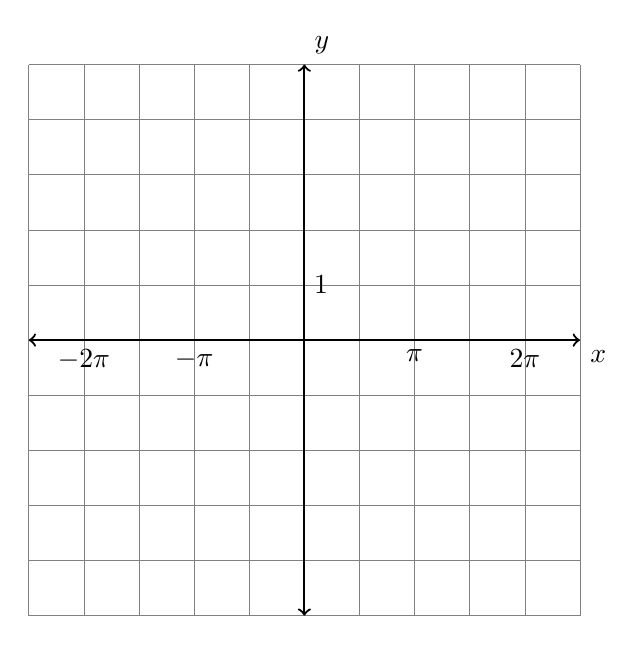
\begin{tikzpicture}[scale=0.7]
    \plane
    \end{tikzpicture}
\end{figure}
\question Sketch the graph of $-2\cos(x)-2.$
\begin{figure}[h]
\centering
    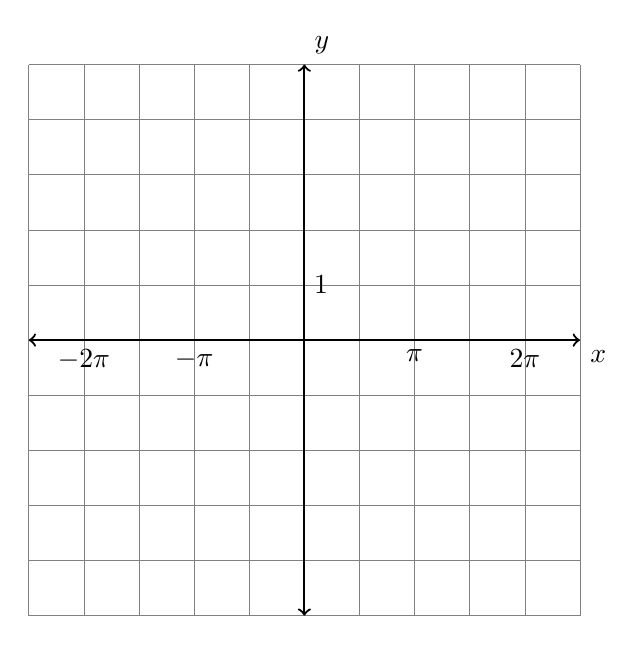
\begin{tikzpicture}[scale=0.7]
    \plane
    \end{tikzpicture}
\end{figure}
\newpage\subsection*{Quiz ID:301}
\question Using your calculator, find $\sin 1.6$
     \question Using your calculator find $\cos 33.2^{\circ}$
\question For an angle $\theta$ in quadrant I , if $ \cos\theta=\dfrac{4}{\sqrt{20}}$ find $ \csc\theta $\makeemptybox{\stretch{1}}
\begin{table}[b]
\centering
\begin{tabular}{|l|l|l|l|l|l|l|}
\hline
\textbf{Question} & 1(/20) & 2(/20) & 3(/20) & 4(/20) & 5(/20) & \textbf{Total (/100)} \\ \hline
\textbf{Score}    &        &        &        &        &        &                      \\ \hline
\end{tabular}
\end{table}
\end{questions}\newpage
\section*{Quiz 45}
\subsection*{Quiz ID: 302}
\makebox[0.4\textwidth]{English Name:\enspace\hrulefill}
\vspace{0.5cm}\
\makebox[0.4\textwidth]{Chinese Name:\enspace\hrulefill}
\vspace{1cm}\
\begin{questions}
\question Sketch the graph of $4\sin(x)+1$.
\begin{figure}[h]
\centering
    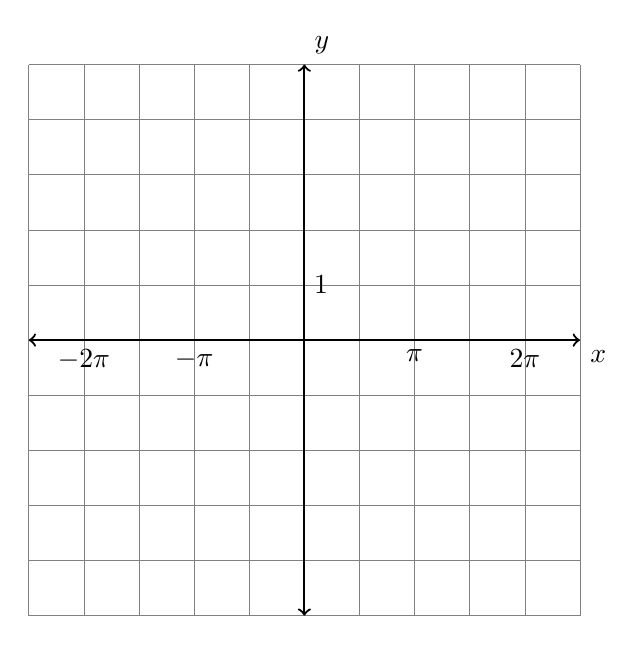
\begin{tikzpicture}[scale=0.7]
    \plane
    \end{tikzpicture}
\end{figure}
\question Sketch the graph of $-3\cos(x)-2.$
\begin{figure}[h]
\centering
    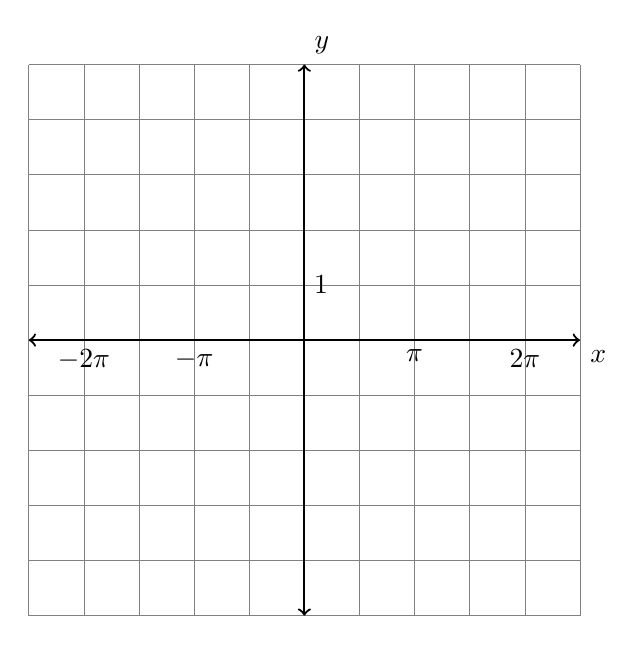
\begin{tikzpicture}[scale=0.7]
    \plane
    \end{tikzpicture}
\end{figure}
\newpage\subsection*{Quiz ID:302}
\question Using your calculator, find $\sin 4.75$
     \question Using your calculator find $\cos 49.65^{\circ}$
\question For an angle $\theta$ in quadrant I , if $ \csc\theta=\dfrac{\sqrt{61}}{5}$ find $ \sin\theta $\makeemptybox{\stretch{1}}
\begin{table}[b]
\centering
\begin{tabular}{|l|l|l|l|l|l|l|}
\hline
\textbf{Question} & 1(/20) & 2(/20) & 3(/20) & 4(/20) & 5(/20) & \textbf{Total (/100)} \\ \hline
\textbf{Score}    &        &        &        &        &        &                      \\ \hline
\end{tabular}
\end{table}
\end{questions}\newpage
\section*{Quiz 45}
\subsection*{Quiz ID: 303}
\makebox[0.4\textwidth]{English Name:\enspace\hrulefill}
\vspace{0.5cm}\
\makebox[0.4\textwidth]{Chinese Name:\enspace\hrulefill}
\vspace{1cm}\
\begin{questions}
\question Sketch the graph of $4\sin(x)+1$.
\begin{figure}[h]
\centering
    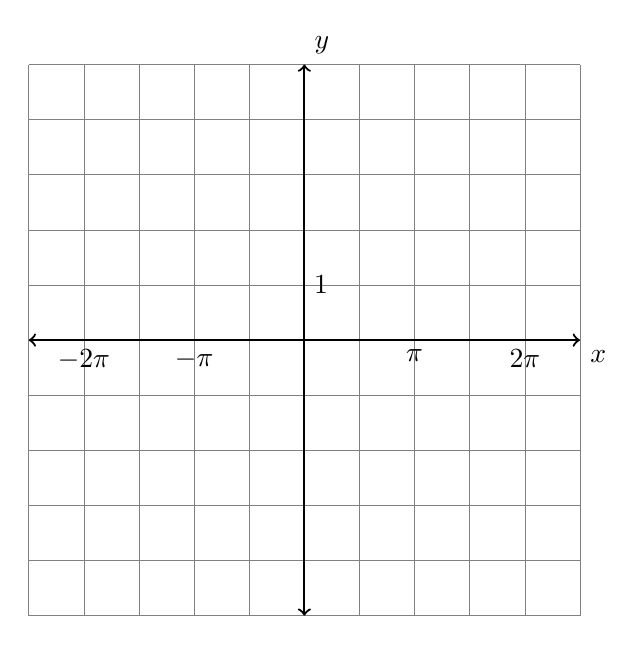
\begin{tikzpicture}[scale=0.7]
    \plane
    \end{tikzpicture}
\end{figure}
\question Sketch the graph of $-4\cos(x)-1.$
\begin{figure}[h]
\centering
    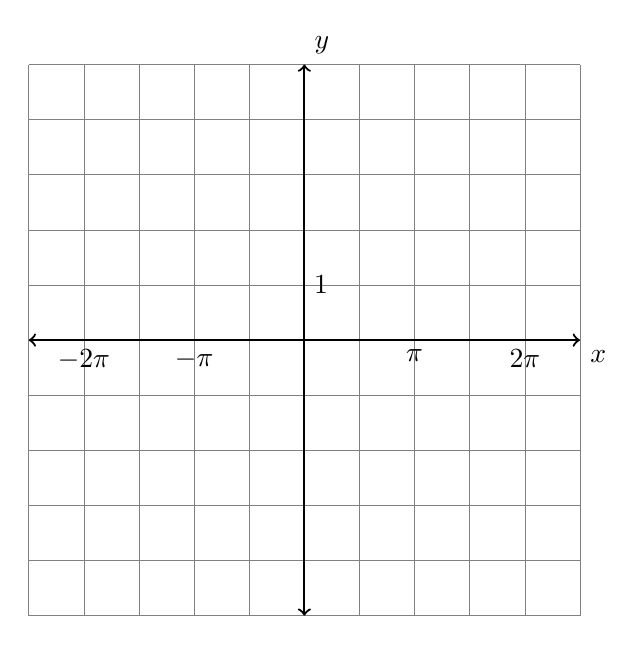
\begin{tikzpicture}[scale=0.7]
    \plane
    \end{tikzpicture}
\end{figure}
\newpage\subsection*{Quiz ID:303}
\question Using your calculator, find $\sin 0.2$
     \question Using your calculator find $\cos 19.1^{\circ}$
\question For an angle $\theta$ in quadrant I , if $ \tan\theta=\dfrac{5}{6}$ find $ \cos\theta $\makeemptybox{\stretch{1}}
\begin{table}[b]
\centering
\begin{tabular}{|l|l|l|l|l|l|l|}
\hline
\textbf{Question} & 1(/20) & 2(/20) & 3(/20) & 4(/20) & 5(/20) & \textbf{Total (/100)} \\ \hline
\textbf{Score}    &        &        &        &        &        &                      \\ \hline
\end{tabular}
\end{table}
\end{questions}\newpage
\section*{Quiz 45}
\subsection*{Quiz ID: 304}
\makebox[0.4\textwidth]{English Name:\enspace\hrulefill}
\vspace{0.5cm}\
\makebox[0.4\textwidth]{Chinese Name:\enspace\hrulefill}
\vspace{1cm}\
\begin{questions}
\question Sketch the graph of $3\sin(x)+2$.
\begin{figure}[h]
\centering
    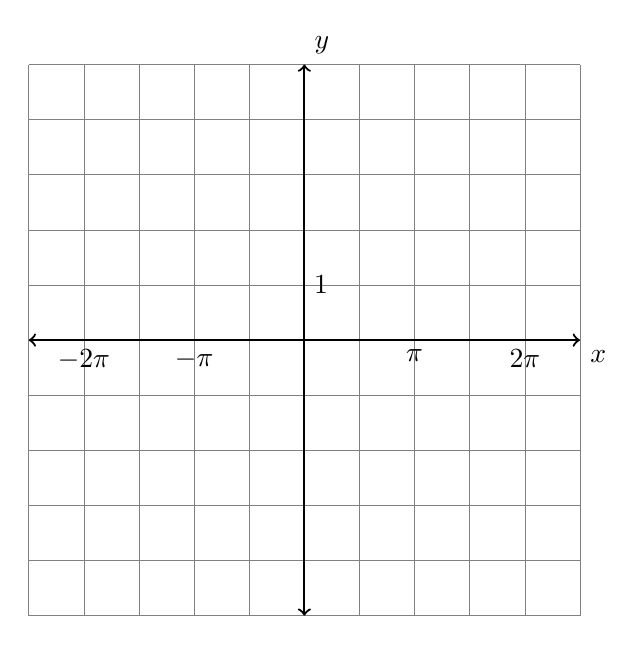
\begin{tikzpicture}[scale=0.7]
    \plane
    \end{tikzpicture}
\end{figure}
\question Sketch the graph of $-4\cos(x)-1.$
\begin{figure}[h]
\centering
    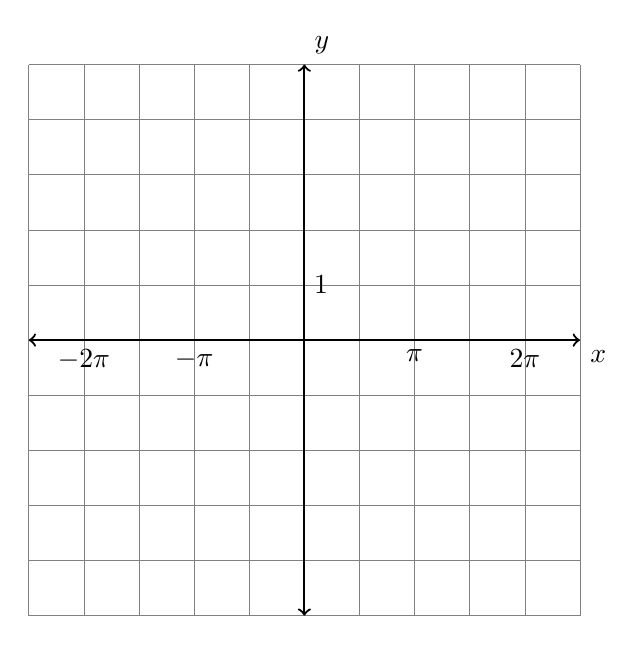
\begin{tikzpicture}[scale=0.7]
    \plane
    \end{tikzpicture}
\end{figure}
\newpage\subsection*{Quiz ID:304}
\question Using your calculator, find $\sin 2.3$
     \question Using your calculator find $\cos 129.55^{\circ}$
\question For an angle $\theta$ in quadrant I , if $ \csc\theta=\dfrac{\sqrt{13}}{2}$ find $ \cos\theta $\makeemptybox{\stretch{1}}
\begin{table}[b]
\centering
\begin{tabular}{|l|l|l|l|l|l|l|}
\hline
\textbf{Question} & 1(/20) & 2(/20) & 3(/20) & 4(/20) & 5(/20) & \textbf{Total (/100)} \\ \hline
\textbf{Score}    &        &        &        &        &        &                      \\ \hline
\end{tabular}
\end{table}
\end{questions}\newpage
\section*{Quiz 45}
\subsection*{Quiz ID: 305}
\makebox[0.4\textwidth]{English Name:\enspace\hrulefill}
\vspace{0.5cm}\
\makebox[0.4\textwidth]{Chinese Name:\enspace\hrulefill}
\vspace{1cm}\
\begin{questions}
\question Sketch the graph of $4\sin(x)+1$.
\begin{figure}[h]
\centering
    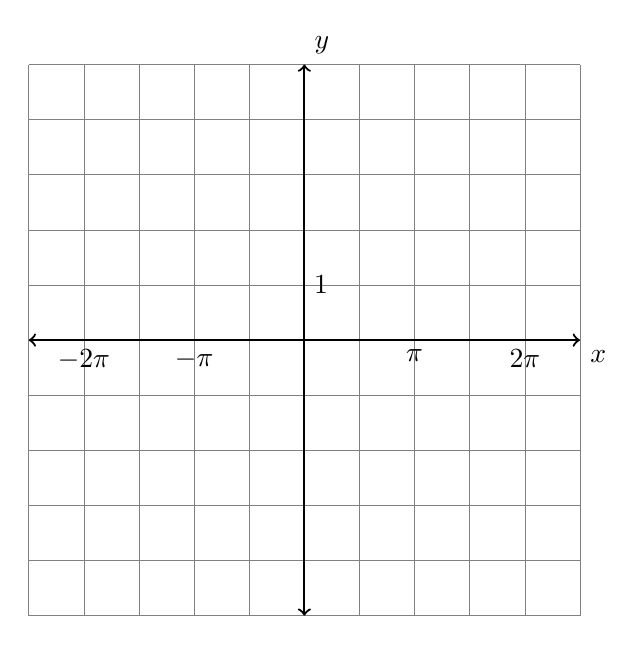
\begin{tikzpicture}[scale=0.7]
    \plane
    \end{tikzpicture}
\end{figure}
\question Sketch the graph of $-3\cos(x)-2.$
\begin{figure}[h]
\centering
    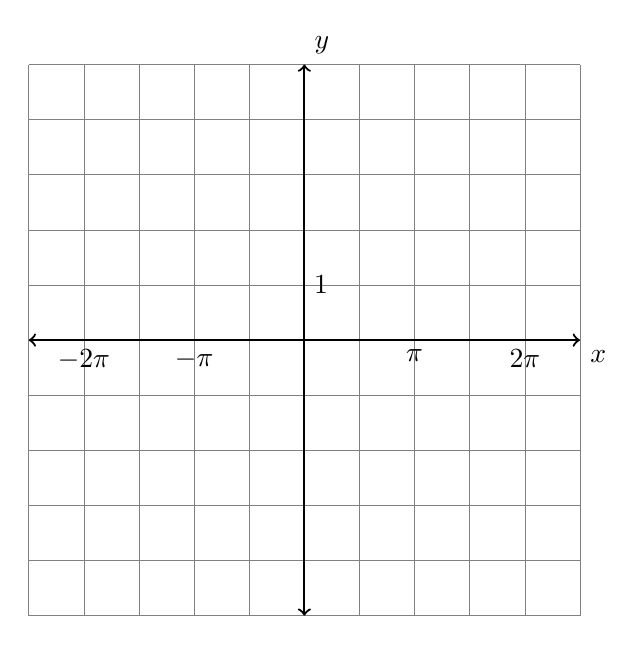
\begin{tikzpicture}[scale=0.7]
    \plane
    \end{tikzpicture}
\end{figure}
\newpage\subsection*{Quiz ID:305}
\question Using your calculator, find $\sin 3.35$
     \question Using your calculator find $\cos 101.35^{\circ}$
\question For an angle $\theta$ in quadrant I , if $ \cot\theta=\dfrac{3}{2}$ find $ \tan\theta $\makeemptybox{\stretch{1}}
\begin{table}[b]
\centering
\begin{tabular}{|l|l|l|l|l|l|l|}
\hline
\textbf{Question} & 1(/20) & 2(/20) & 3(/20) & 4(/20) & 5(/20) & \textbf{Total (/100)} \\ \hline
\textbf{Score}    &        &        &        &        &        &                      \\ \hline
\end{tabular}
\end{table}
\end{questions}\newpage
\section*{Quiz 45}
\subsection*{Quiz ID: 306}
\makebox[0.4\textwidth]{English Name:\enspace\hrulefill}
\vspace{0.5cm}\
\makebox[0.4\textwidth]{Chinese Name:\enspace\hrulefill}
\vspace{1cm}\
\begin{questions}
\question Sketch the graph of $2\sin(x)+2$.
\begin{figure}[h]
\centering
    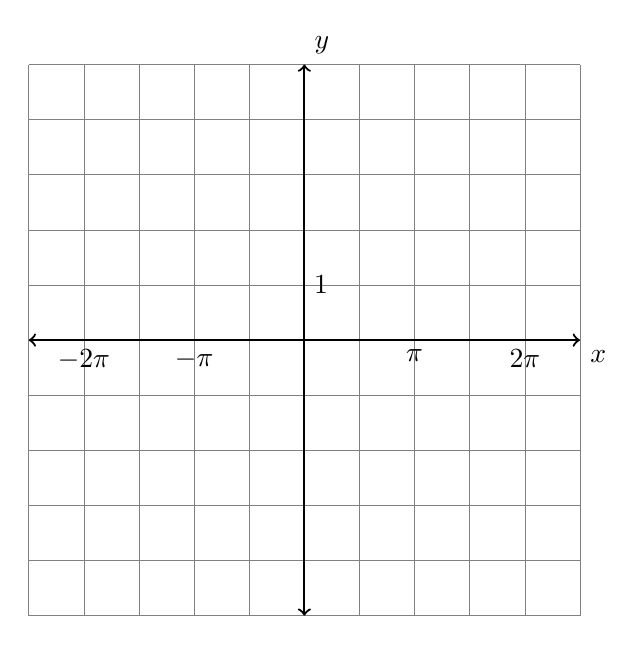
\begin{tikzpicture}[scale=0.7]
    \plane
    \end{tikzpicture}
\end{figure}
\question Sketch the graph of $-4\cos(x)-1.$
\begin{figure}[h]
\centering
    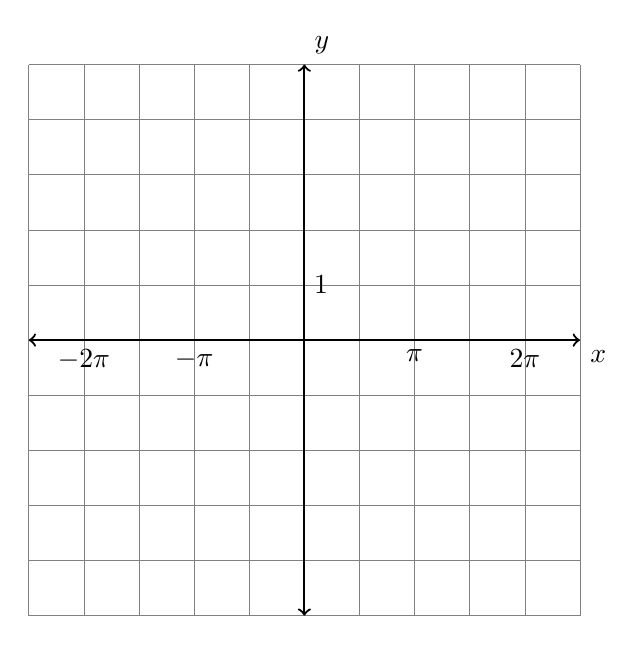
\begin{tikzpicture}[scale=0.7]
    \plane
    \end{tikzpicture}
\end{figure}
\newpage\subsection*{Quiz ID:306}
\question Using your calculator, find $\sin 4.05$
     \question Using your calculator find $\cos 12.05^{\circ}$
\question For an angle $\theta$ in quadrant I , if $ \sin\theta=\dfrac{2}{\sqrt{20}}$ find $ \cot\theta $\makeemptybox{\stretch{1}}
\begin{table}[b]
\centering
\begin{tabular}{|l|l|l|l|l|l|l|}
\hline
\textbf{Question} & 1(/20) & 2(/20) & 3(/20) & 4(/20) & 5(/20) & \textbf{Total (/100)} \\ \hline
\textbf{Score}    &        &        &        &        &        &                      \\ \hline
\end{tabular}
\end{table}
\end{questions}\newpage
\section*{Quiz 45}
\subsection*{Quiz ID: 307}
\makebox[0.4\textwidth]{English Name:\enspace\hrulefill}
\vspace{0.5cm}\
\makebox[0.4\textwidth]{Chinese Name:\enspace\hrulefill}
\vspace{1cm}\
\begin{questions}
\question Sketch the graph of $2\sin(x)+1$.
\begin{figure}[h]
\centering
    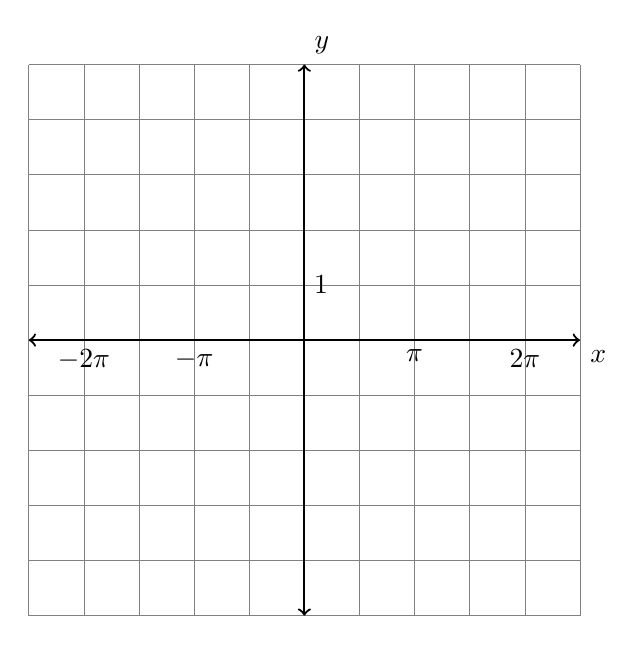
\begin{tikzpicture}[scale=0.7]
    \plane
    \end{tikzpicture}
\end{figure}
\question Sketch the graph of $-3\cos(x)-2.$
\begin{figure}[h]
\centering
    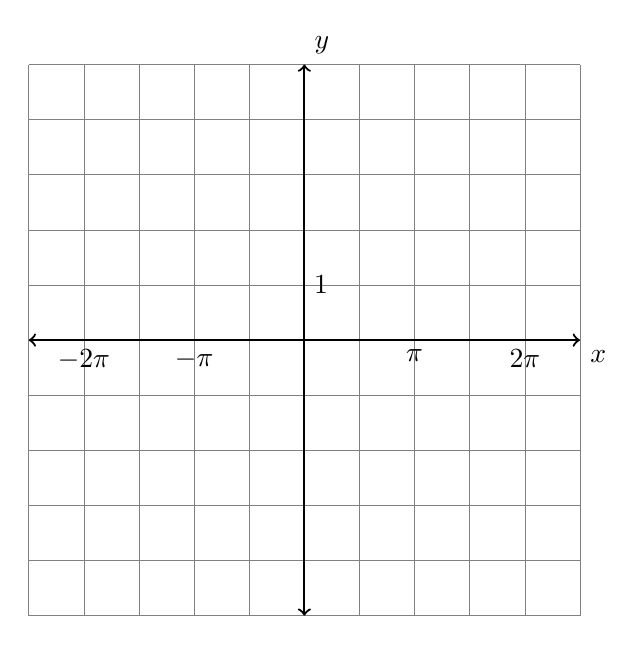
\begin{tikzpicture}[scale=0.7]
    \plane
    \end{tikzpicture}
\end{figure}
\newpage\subsection*{Quiz ID:307}
\question Using your calculator, find $\sin 5.1$
     \question Using your calculator find $\cos 77.85^{\circ}$
\question For an angle $\theta$ in quadrant I , if $ \csc\theta=\dfrac{\sqrt{41}}{4}$ find $ \cot\theta $\makeemptybox{\stretch{1}}
\begin{table}[b]
\centering
\begin{tabular}{|l|l|l|l|l|l|l|}
\hline
\textbf{Question} & 1(/20) & 2(/20) & 3(/20) & 4(/20) & 5(/20) & \textbf{Total (/100)} \\ \hline
\textbf{Score}    &        &        &        &        &        &                      \\ \hline
\end{tabular}
\end{table}
\end{questions}\newpage
\section*{Quiz 45}
\subsection*{Quiz ID: 308}
\makebox[0.4\textwidth]{English Name:\enspace\hrulefill}
\vspace{0.5cm}\
\makebox[0.4\textwidth]{Chinese Name:\enspace\hrulefill}
\vspace{1cm}\
\begin{questions}
\question Sketch the graph of $4\sin(x)+1$.
\begin{figure}[h]
\centering
    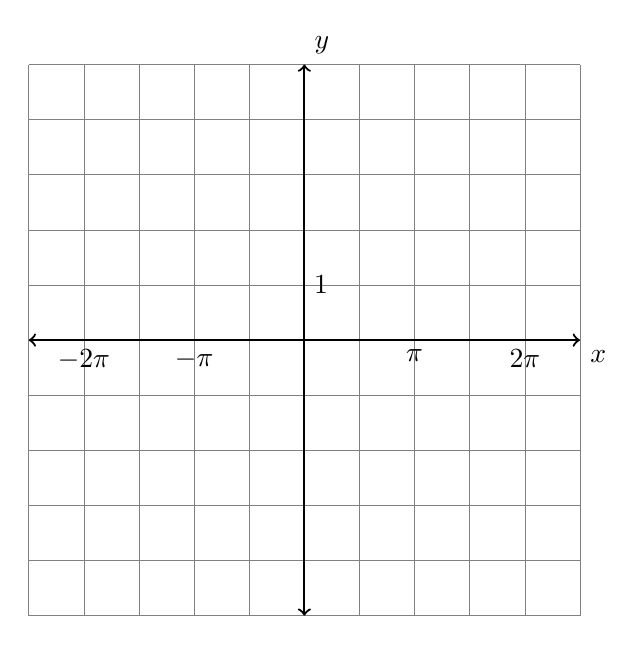
\begin{tikzpicture}[scale=0.7]
    \plane
    \end{tikzpicture}
\end{figure}
\question Sketch the graph of $-2\cos(x)-3.$
\begin{figure}[h]
\centering
    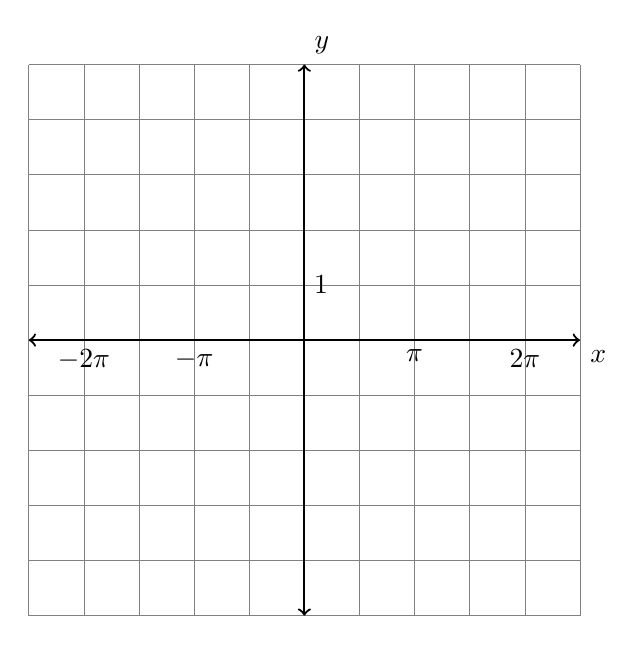
\begin{tikzpicture}[scale=0.7]
    \plane
    \end{tikzpicture}
\end{figure}
\newpage\subsection*{Quiz ID:308}
\question Using your calculator, find $\sin 5.1$
     \question Using your calculator find $\cos 185.95^{\circ}$
\question For an angle $\theta$ in quadrant I , if $ \sin\theta=\dfrac{2}{\sqrt{13}}$ find $ \sec\theta $\makeemptybox{\stretch{1}}
\begin{table}[b]
\centering
\begin{tabular}{|l|l|l|l|l|l|l|}
\hline
\textbf{Question} & 1(/20) & 2(/20) & 3(/20) & 4(/20) & 5(/20) & \textbf{Total (/100)} \\ \hline
\textbf{Score}    &        &        &        &        &        &                      \\ \hline
\end{tabular}
\end{table}
\end{questions}\newpage
\section*{Quiz 45}
\subsection*{Quiz ID: 309}
\makebox[0.4\textwidth]{English Name:\enspace\hrulefill}
\vspace{0.5cm}\
\makebox[0.4\textwidth]{Chinese Name:\enspace\hrulefill}
\vspace{1cm}\
\begin{questions}
\question Sketch the graph of $2\sin(x)+3$.
\begin{figure}[h]
\centering
    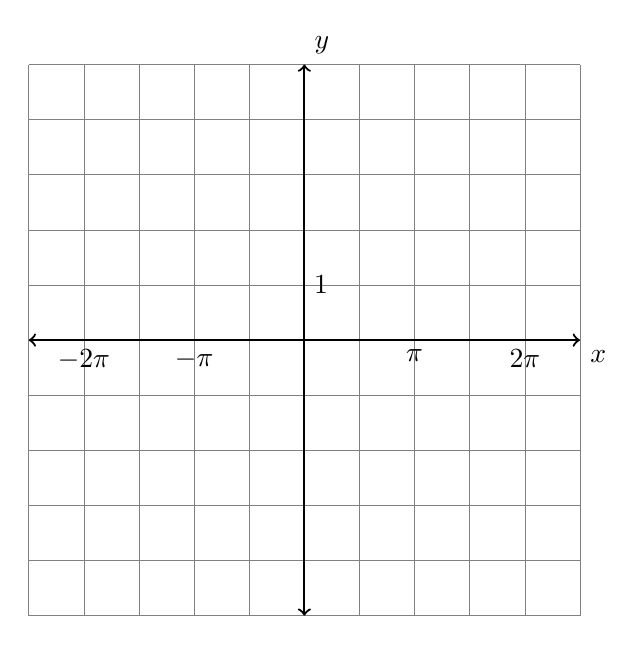
\begin{tikzpicture}[scale=0.7]
    \plane
    \end{tikzpicture}
\end{figure}
\question Sketch the graph of $-4\cos(x)-1.$
\begin{figure}[h]
\centering
    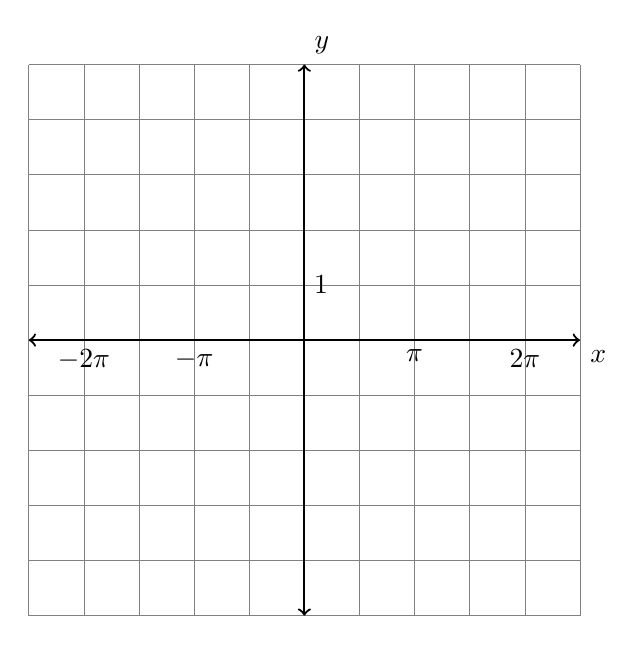
\begin{tikzpicture}[scale=0.7]
    \plane
    \end{tikzpicture}
\end{figure}
\newpage\subsection*{Quiz ID:309}
\question Using your calculator, find $\sin 1.25$
     \question Using your calculator find $\cos 56.7^{\circ}$
\question For an angle $\theta$ in quadrant I , if $ \sin\theta=\dfrac{2}{\sqrt{20}}$ find $ \tan\theta $\makeemptybox{\stretch{1}}
\begin{table}[b]
\centering
\begin{tabular}{|l|l|l|l|l|l|l|}
\hline
\textbf{Question} & 1(/20) & 2(/20) & 3(/20) & 4(/20) & 5(/20) & \textbf{Total (/100)} \\ \hline
\textbf{Score}    &        &        &        &        &        &                      \\ \hline
\end{tabular}
\end{table}
\end{questions}\newpage
\section*{Quiz 45}
\subsection*{Quiz ID: 310}
\makebox[0.4\textwidth]{English Name:\enspace\hrulefill}
\vspace{0.5cm}\
\makebox[0.4\textwidth]{Chinese Name:\enspace\hrulefill}
\vspace{1cm}\
\begin{questions}
\question Sketch the graph of $4\sin(x)+1$.
\begin{figure}[h]
\centering
    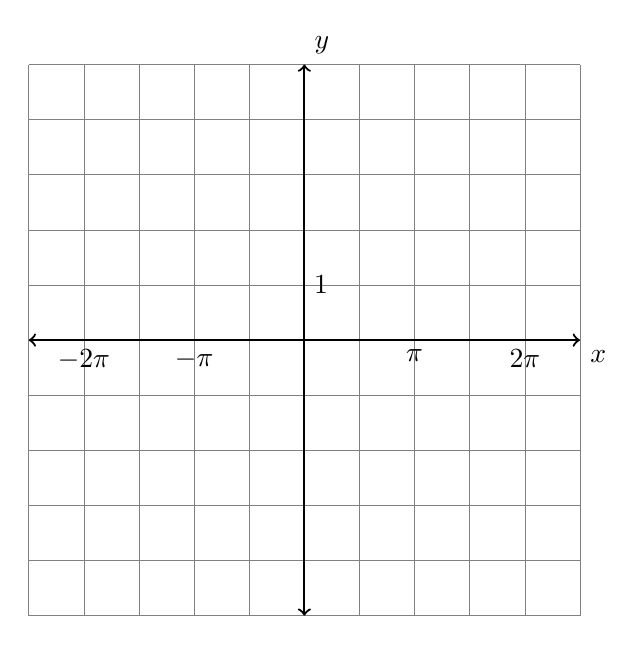
\begin{tikzpicture}[scale=0.7]
    \plane
    \end{tikzpicture}
\end{figure}
\question Sketch the graph of $-3\cos(x)-1.$
\begin{figure}[h]
\centering
    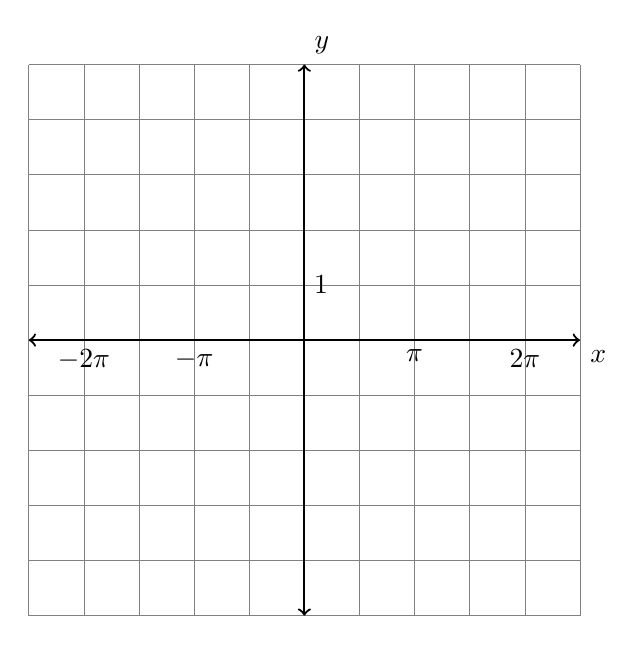
\begin{tikzpicture}[scale=0.7]
    \plane
    \end{tikzpicture}
\end{figure}
\newpage\subsection*{Quiz ID:310}
\question Using your calculator, find $\sin 2.3$
     \question Using your calculator find $\cos 63.75^{\circ}$
\question For an angle $\theta$ in quadrant I , if $ \cot\theta=\dfrac{4}{3}$ find $ \csc\theta $\makeemptybox{\stretch{1}}
\begin{table}[b]
\centering
\begin{tabular}{|l|l|l|l|l|l|l|}
\hline
\textbf{Question} & 1(/20) & 2(/20) & 3(/20) & 4(/20) & 5(/20) & \textbf{Total (/100)} \\ \hline
\textbf{Score}    &        &        &        &        &        &                      \\ \hline
\end{tabular}
\end{table}
\end{questions}\newpage
\section*{Quiz 45}
\subsection*{Quiz ID: 311}
\makebox[0.4\textwidth]{English Name:\enspace\hrulefill}
\vspace{0.5cm}\
\makebox[0.4\textwidth]{Chinese Name:\enspace\hrulefill}
\vspace{1cm}\
\begin{questions}
\question Sketch the graph of $2\sin(x)+2$.
\begin{figure}[h]
\centering
    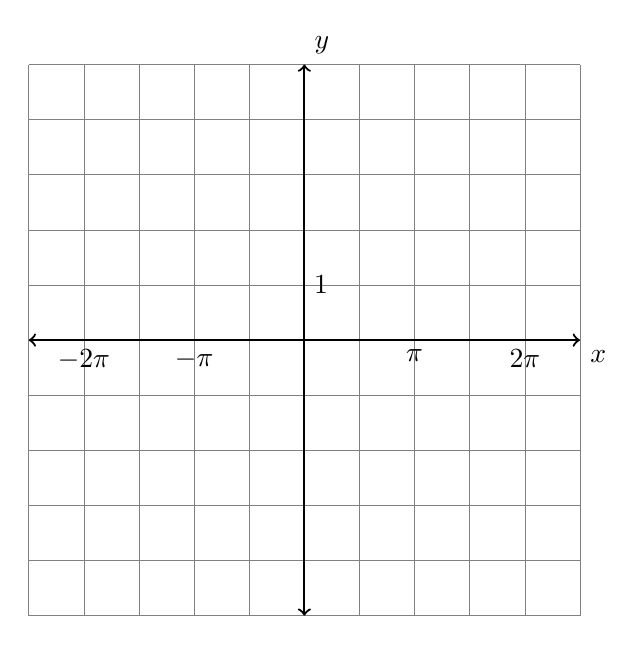
\begin{tikzpicture}[scale=0.7]
    \plane
    \end{tikzpicture}
\end{figure}
\question Sketch the graph of $-4\cos(x)-1.$
\begin{figure}[h]
\centering
    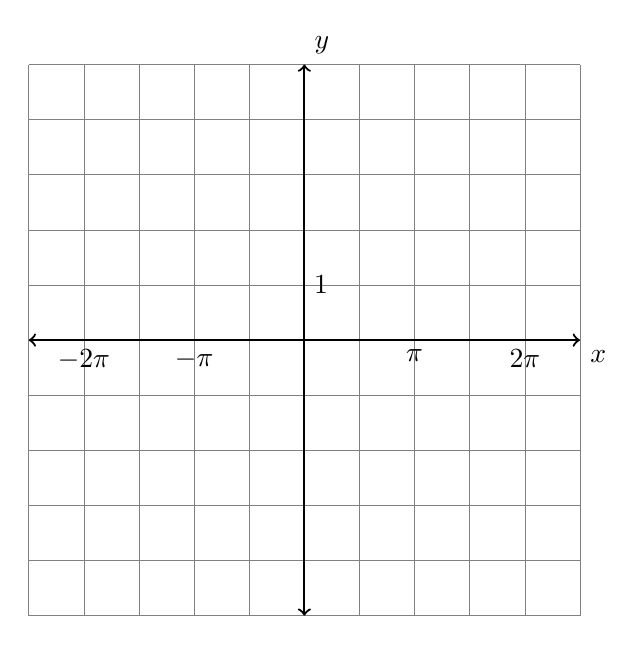
\begin{tikzpicture}[scale=0.7]
    \plane
    \end{tikzpicture}
\end{figure}
\newpage\subsection*{Quiz ID:311}
\question Using your calculator, find $\sin 3.7$
     \question Using your calculator find $\cos 59.05^{\circ}$
\question For an angle $\theta$ in quadrant I , if $ \cos\theta=\dfrac{5}{\sqrt{34}}$ find $ \sin\theta $\makeemptybox{\stretch{1}}
\begin{table}[b]
\centering
\begin{tabular}{|l|l|l|l|l|l|l|}
\hline
\textbf{Question} & 1(/20) & 2(/20) & 3(/20) & 4(/20) & 5(/20) & \textbf{Total (/100)} \\ \hline
\textbf{Score}    &        &        &        &        &        &                      \\ \hline
\end{tabular}
\end{table}
\end{questions}\newpage
\section*{Quiz 45}
\subsection*{Quiz ID: 312}
\makebox[0.4\textwidth]{English Name:\enspace\hrulefill}
\vspace{0.5cm}\
\makebox[0.4\textwidth]{Chinese Name:\enspace\hrulefill}
\vspace{1cm}\
\begin{questions}
\question Sketch the graph of $2\sin(x)+2$.
\begin{figure}[h]
\centering
    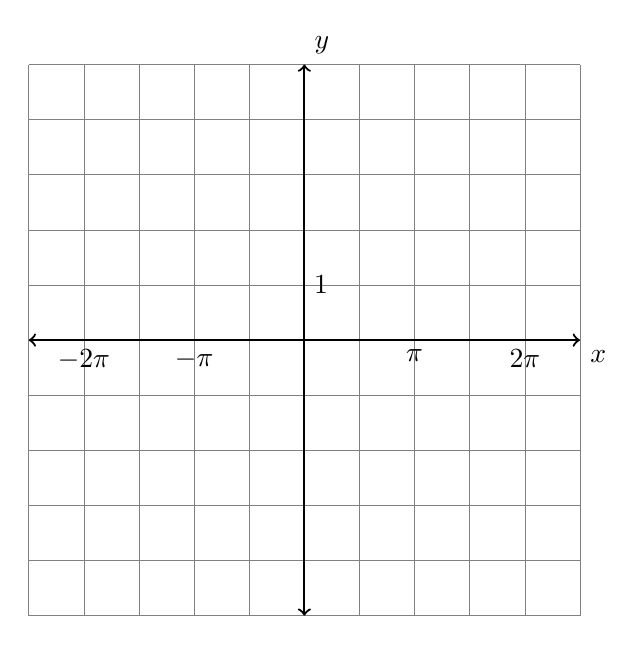
\begin{tikzpicture}[scale=0.7]
    \plane
    \end{tikzpicture}
\end{figure}
\question Sketch the graph of $-4\cos(x)-1.$
\begin{figure}[h]
\centering
    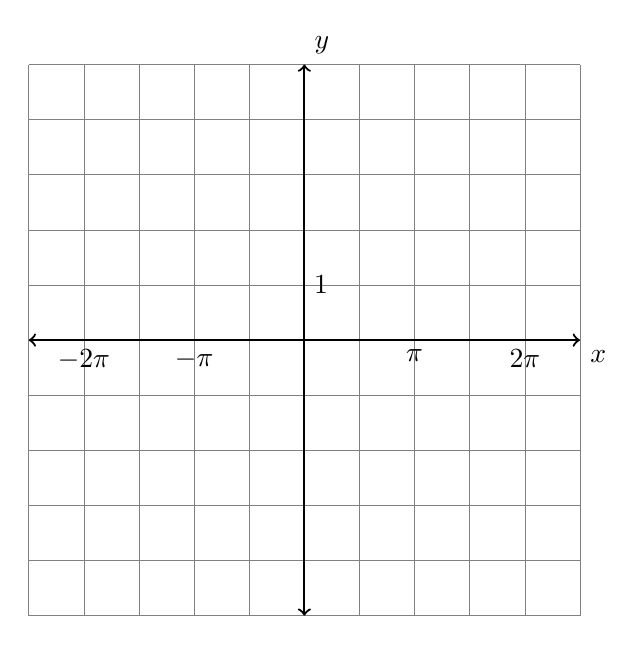
\begin{tikzpicture}[scale=0.7]
    \plane
    \end{tikzpicture}
\end{figure}
\newpage\subsection*{Quiz ID:312}
\question Using your calculator, find $\sin 4.75$
     \question Using your calculator find $\cos 84.9^{\circ}$
\question For an angle $\theta$ in quadrant I , if $ \tan\theta=\dfrac{4}{6}$ find $ \sec\theta $\makeemptybox{\stretch{1}}
\begin{table}[b]
\centering
\begin{tabular}{|l|l|l|l|l|l|l|}
\hline
\textbf{Question} & 1(/20) & 2(/20) & 3(/20) & 4(/20) & 5(/20) & \textbf{Total (/100)} \\ \hline
\textbf{Score}    &        &        &        &        &        &                      \\ \hline
\end{tabular}
\end{table}
\end{questions}\newpage
\section*{Quiz 45}
\subsection*{Quiz ID: 313}
\makebox[0.4\textwidth]{English Name:\enspace\hrulefill}
\vspace{0.5cm}\
\makebox[0.4\textwidth]{Chinese Name:\enspace\hrulefill}
\vspace{1cm}\
\begin{questions}
\question Sketch the graph of $3\sin(x)+2$.
\begin{figure}[h]
\centering
    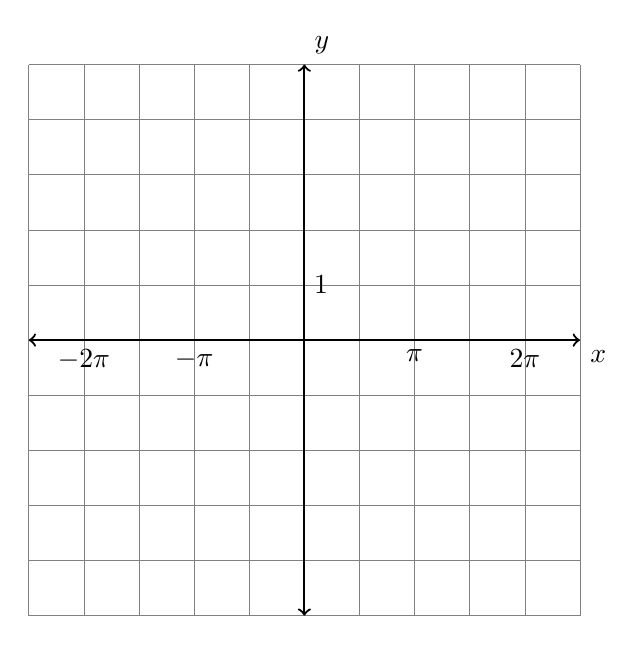
\begin{tikzpicture}[scale=0.7]
    \plane
    \end{tikzpicture}
\end{figure}
\question Sketch the graph of $-3\cos(x)-2.$
\begin{figure}[h]
\centering
    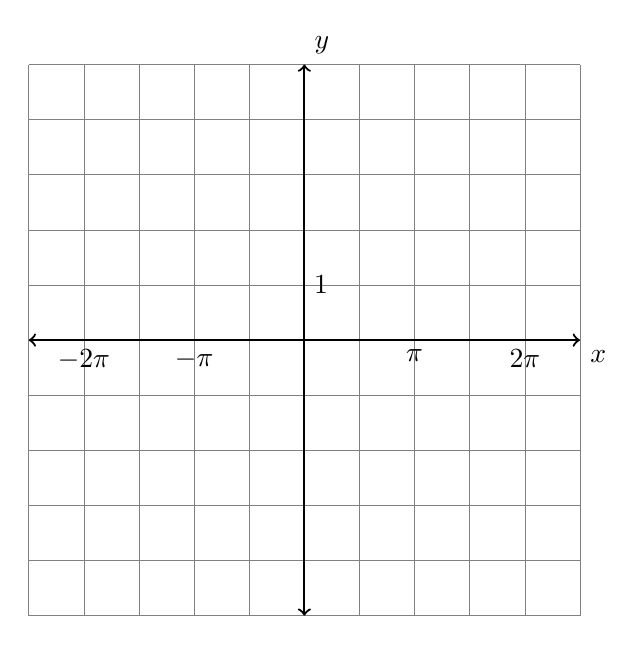
\begin{tikzpicture}[scale=0.7]
    \plane
    \end{tikzpicture}
\end{figure}
\newpage\subsection*{Quiz ID:313}
\question Using your calculator, find $\sin 0.2$
     \question Using your calculator find $\cos 80.2^{\circ}$
\question For an angle $\theta$ in quadrant I , if $ \cot\theta=\dfrac{3}{2}$ find $ \sin\theta $\makeemptybox{\stretch{1}}
\begin{table}[b]
\centering
\begin{tabular}{|l|l|l|l|l|l|l|}
\hline
\textbf{Question} & 1(/20) & 2(/20) & 3(/20) & 4(/20) & 5(/20) & \textbf{Total (/100)} \\ \hline
\textbf{Score}    &        &        &        &        &        &                      \\ \hline
\end{tabular}
\end{table}
\end{questions}\newpage
\section*{Quiz 45}
\subsection*{Quiz ID: 314}
\makebox[0.4\textwidth]{English Name:\enspace\hrulefill}
\vspace{0.5cm}\
\makebox[0.4\textwidth]{Chinese Name:\enspace\hrulefill}
\vspace{1cm}\
\begin{questions}
\question Sketch the graph of $2\sin(x)+2$.
\begin{figure}[h]
\centering
    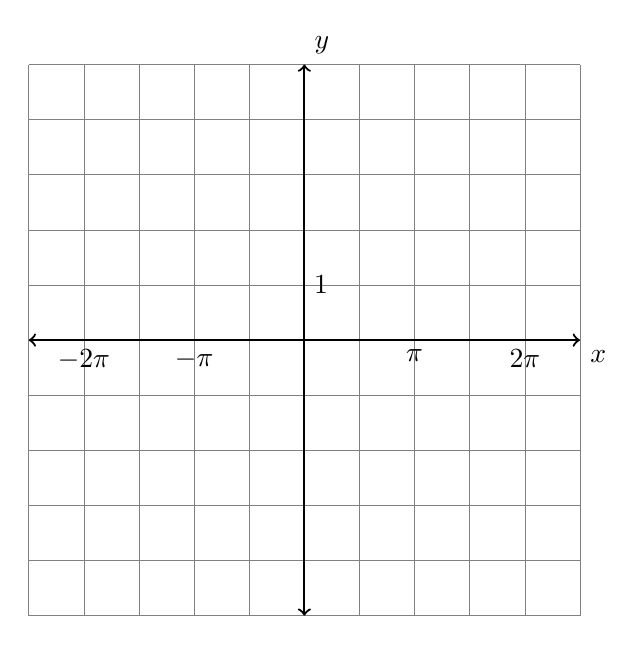
\begin{tikzpicture}[scale=0.7]
    \plane
    \end{tikzpicture}
\end{figure}
\question Sketch the graph of $-2\cos(x)-1.$
\begin{figure}[h]
\centering
    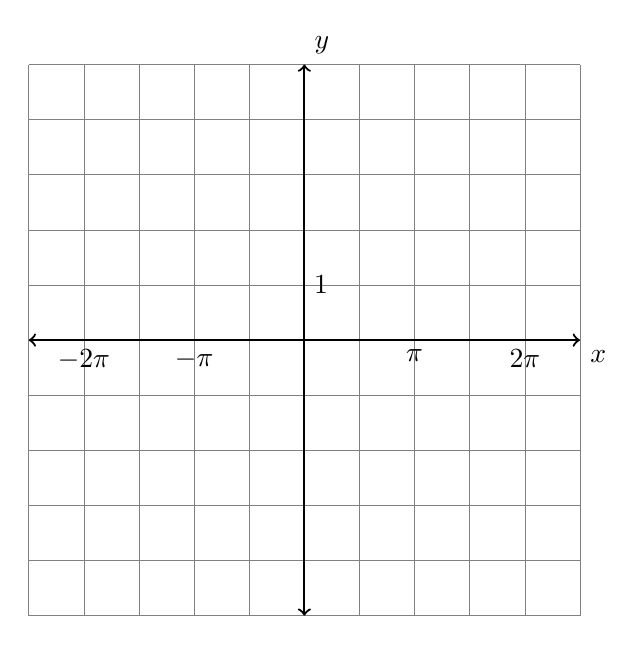
\begin{tikzpicture}[scale=0.7]
    \plane
    \end{tikzpicture}
\end{figure}
\newpage\subsection*{Quiz ID:314}
\question Using your calculator, find $\sin 4.75$
     \question Using your calculator find $\cos 171.85^{\circ}$
\question For an angle $\theta$ in quadrant I , if $ \tan\theta=\dfrac{2}{5}$ find $ \sin\theta $\makeemptybox{\stretch{1}}
\begin{table}[b]
\centering
\begin{tabular}{|l|l|l|l|l|l|l|}
\hline
\textbf{Question} & 1(/20) & 2(/20) & 3(/20) & 4(/20) & 5(/20) & \textbf{Total (/100)} \\ \hline
\textbf{Score}    &        &        &        &        &        &                      \\ \hline
\end{tabular}
\end{table}
\end{questions}\newpage
\section*{Quiz 45}
\subsection*{Quiz ID: 315}
\makebox[0.4\textwidth]{English Name:\enspace\hrulefill}
\vspace{0.5cm}\
\makebox[0.4\textwidth]{Chinese Name:\enspace\hrulefill}
\vspace{1cm}\
\begin{questions}
\question Sketch the graph of $2\sin(x)+1$.
\begin{figure}[h]
\centering
    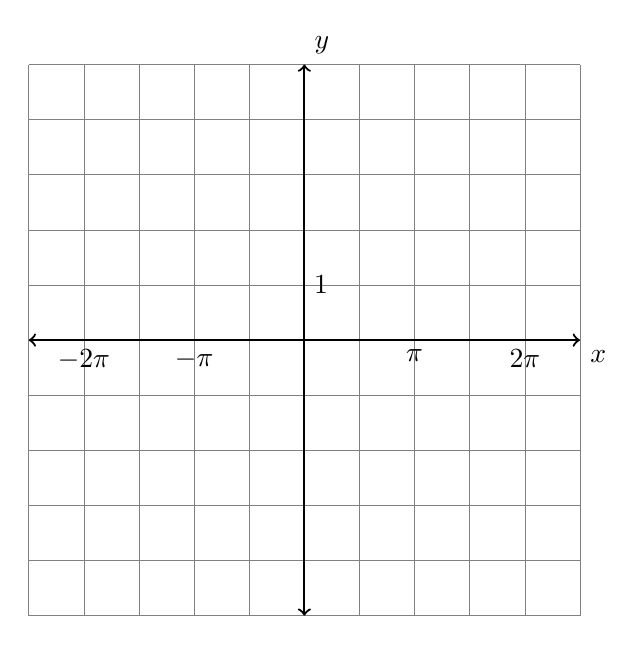
\begin{tikzpicture}[scale=0.7]
    \plane
    \end{tikzpicture}
\end{figure}
\question Sketch the graph of $-3\cos(x)-1.$
\begin{figure}[h]
\centering
    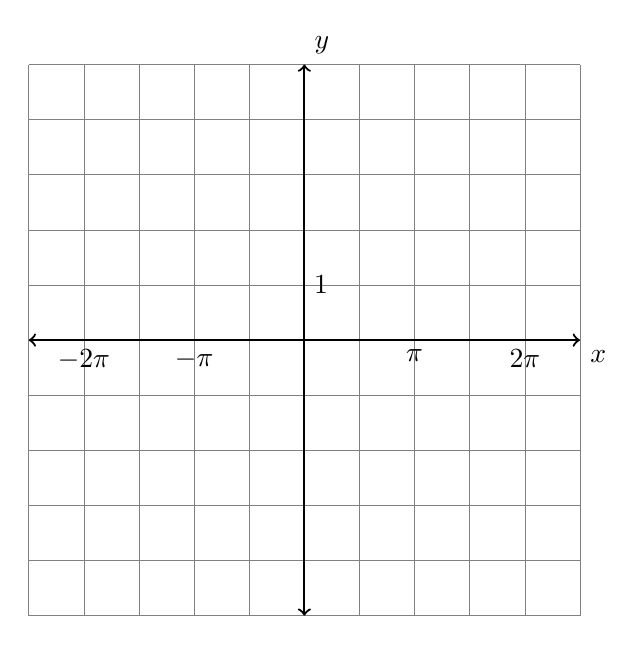
\begin{tikzpicture}[scale=0.7]
    \plane
    \end{tikzpicture}
\end{figure}
\newpage\subsection*{Quiz ID:315}
\question Using your calculator, find $\sin 4.75$
     \question Using your calculator find $\cos 143.65^{\circ}$
\question For an angle $\theta$ in quadrant I , if $ \sec\theta=\dfrac{5}{4}$ find $ \sin\theta $\makeemptybox{\stretch{1}}
\begin{table}[b]
\centering
\begin{tabular}{|l|l|l|l|l|l|l|}
\hline
\textbf{Question} & 1(/20) & 2(/20) & 3(/20) & 4(/20) & 5(/20) & \textbf{Total (/100)} \\ \hline
\textbf{Score}    &        &        &        &        &        &                      \\ \hline
\end{tabular}
\end{table}
\end{questions}\newpage
\section*{Quiz 45}
\subsection*{Quiz ID: 316}
\makebox[0.4\textwidth]{English Name:\enspace\hrulefill}
\vspace{0.5cm}\
\makebox[0.4\textwidth]{Chinese Name:\enspace\hrulefill}
\vspace{1cm}\
\begin{questions}
\question Sketch the graph of $4\sin(x)+1$.
\begin{figure}[h]
\centering
    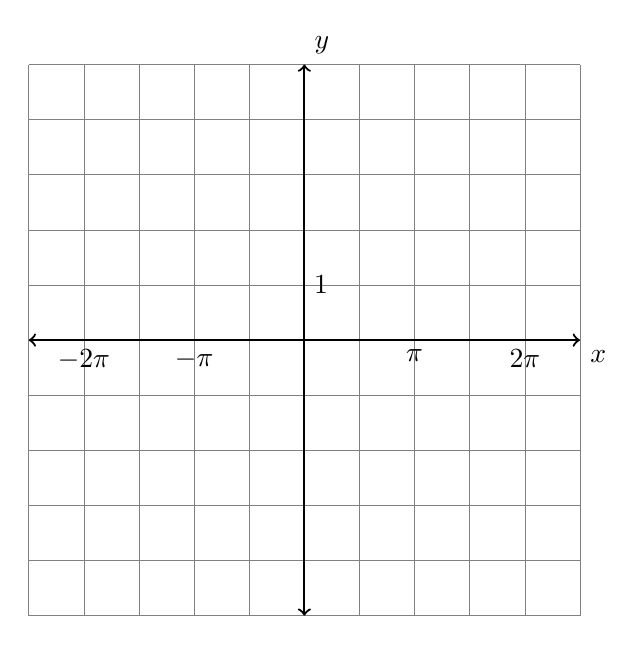
\begin{tikzpicture}[scale=0.7]
    \plane
    \end{tikzpicture}
\end{figure}
\question Sketch the graph of $-2\cos(x)-1.$
\begin{figure}[h]
\centering
    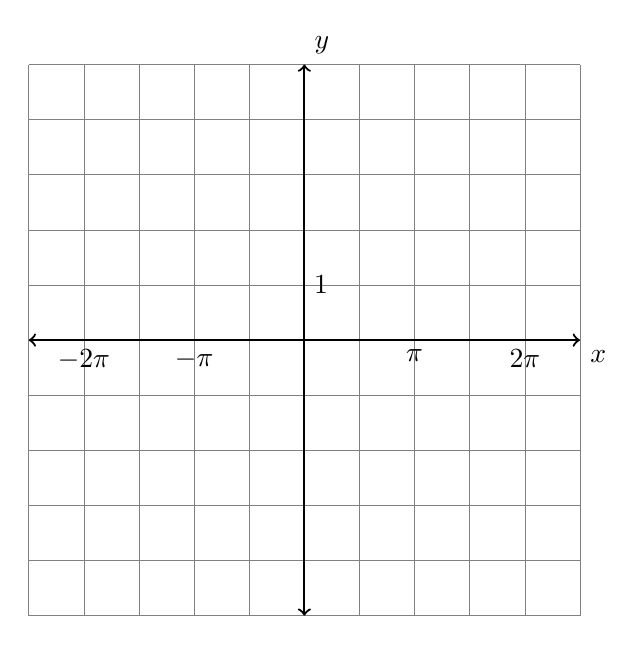
\begin{tikzpicture}[scale=0.7]
    \plane
    \end{tikzpicture}
\end{figure}
\newpage\subsection*{Quiz ID:316}
\question Using your calculator, find $\sin 3.7$
     \question Using your calculator find $\cos 110.75^{\circ}$
\question For an angle $\theta$ in quadrant I , if $ \cot\theta=\dfrac{5}{2}$ find $ \cos\theta $\makeemptybox{\stretch{1}}
\begin{table}[b]
\centering
\begin{tabular}{|l|l|l|l|l|l|l|}
\hline
\textbf{Question} & 1(/20) & 2(/20) & 3(/20) & 4(/20) & 5(/20) & \textbf{Total (/100)} \\ \hline
\textbf{Score}    &        &        &        &        &        &                      \\ \hline
\end{tabular}
\end{table}
\end{questions}\newpage
\section*{Quiz 45}
\subsection*{Quiz ID: 317}
\makebox[0.4\textwidth]{English Name:\enspace\hrulefill}
\vspace{0.5cm}\
\makebox[0.4\textwidth]{Chinese Name:\enspace\hrulefill}
\vspace{1cm}\
\begin{questions}
\question Sketch the graph of $3\sin(x)+2$.
\begin{figure}[h]
\centering
    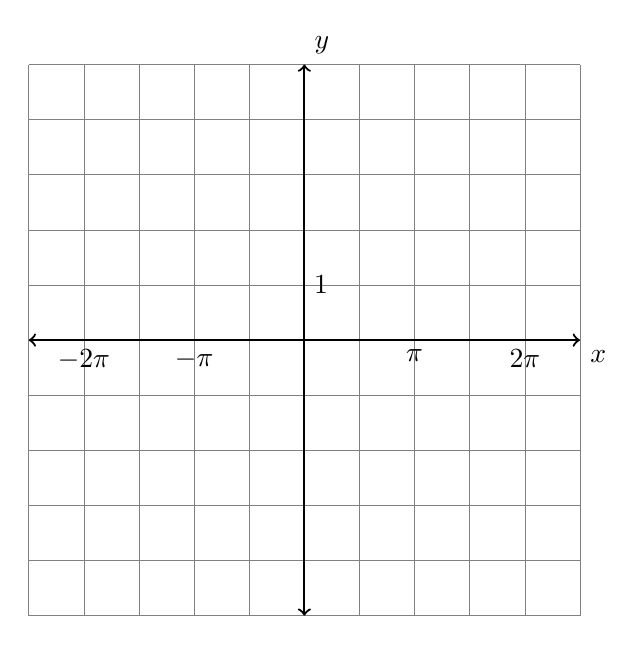
\begin{tikzpicture}[scale=0.7]
    \plane
    \end{tikzpicture}
\end{figure}
\question Sketch the graph of $-4\cos(x)-1.$
\begin{figure}[h]
\centering
    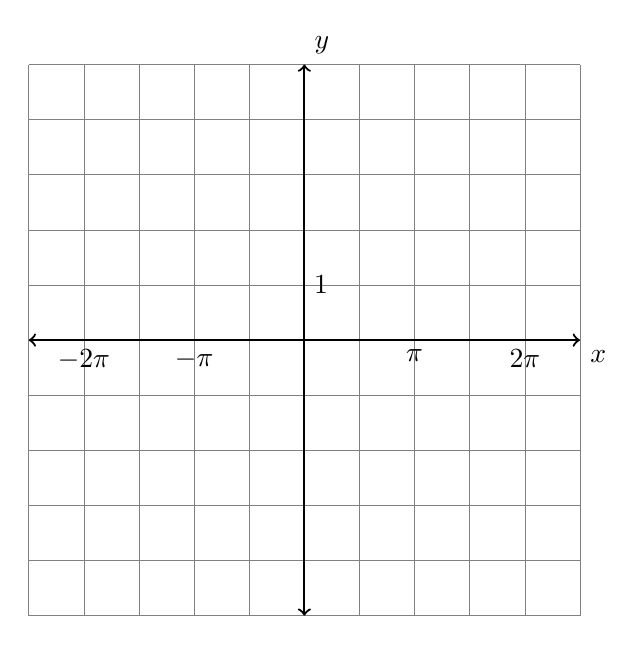
\begin{tikzpicture}[scale=0.7]
    \plane
    \end{tikzpicture}
\end{figure}
\newpage\subsection*{Quiz ID:317}
\question Using your calculator, find $\sin 2.65$
     \question Using your calculator find $\cos 19.1^{\circ}$
\question For an angle $\theta$ in quadrant I , if $ \csc\theta=\dfrac{\sqrt{29}}{2}$ find $ \sin\theta $\makeemptybox{\stretch{1}}
\begin{table}[b]
\centering
\begin{tabular}{|l|l|l|l|l|l|l|}
\hline
\textbf{Question} & 1(/20) & 2(/20) & 3(/20) & 4(/20) & 5(/20) & \textbf{Total (/100)} \\ \hline
\textbf{Score}    &        &        &        &        &        &                      \\ \hline
\end{tabular}
\end{table}
\end{questions}\newpage
\section*{Quiz 45}
\subsection*{Quiz ID: 318}
\makebox[0.4\textwidth]{English Name:\enspace\hrulefill}
\vspace{0.5cm}\
\makebox[0.4\textwidth]{Chinese Name:\enspace\hrulefill}
\vspace{1cm}\
\begin{questions}
\question Sketch the graph of $3\sin(x)+2$.
\begin{figure}[h]
\centering
    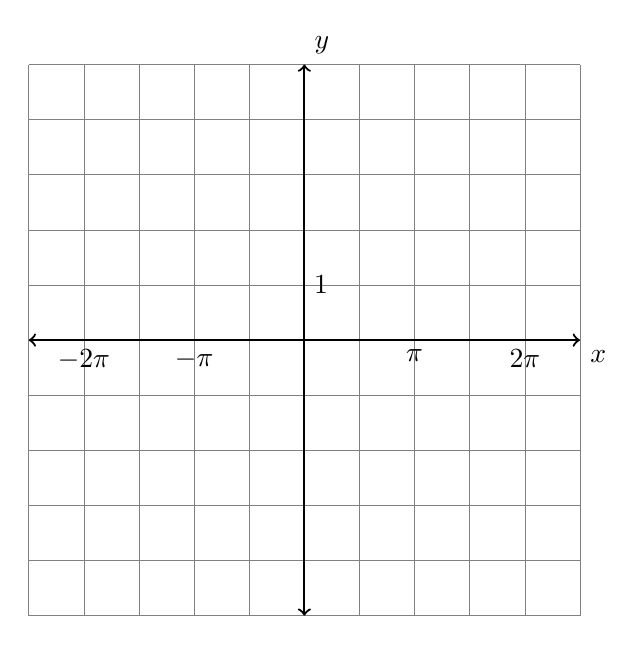
\begin{tikzpicture}[scale=0.7]
    \plane
    \end{tikzpicture}
\end{figure}
\question Sketch the graph of $-4\cos(x)-1.$
\begin{figure}[h]
\centering
    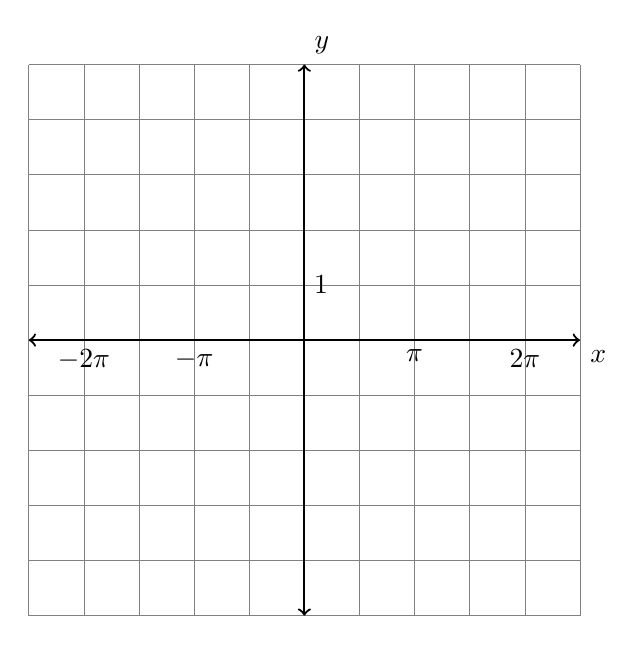
\begin{tikzpicture}[scale=0.7]
    \plane
    \end{tikzpicture}
\end{figure}
\newpage\subsection*{Quiz ID:318}
\question Using your calculator, find $\sin 2.3$
     \question Using your calculator find $\cos 113.1^{\circ}$
\question For an angle $\theta$ in quadrant I , if $ \cot\theta=\dfrac{6}{3}$ find $ \sin\theta $\makeemptybox{\stretch{1}}
\begin{table}[b]
\centering
\begin{tabular}{|l|l|l|l|l|l|l|}
\hline
\textbf{Question} & 1(/20) & 2(/20) & 3(/20) & 4(/20) & 5(/20) & \textbf{Total (/100)} \\ \hline
\textbf{Score}    &        &        &        &        &        &                      \\ \hline
\end{tabular}
\end{table}
\end{questions}\newpage
\section*{Quiz 45}
\subsection*{Quiz ID: 319}
\makebox[0.4\textwidth]{English Name:\enspace\hrulefill}
\vspace{0.5cm}\
\makebox[0.4\textwidth]{Chinese Name:\enspace\hrulefill}
\vspace{1cm}\
\begin{questions}
\question Sketch the graph of $3\sin(x)+2$.
\begin{figure}[h]
\centering
    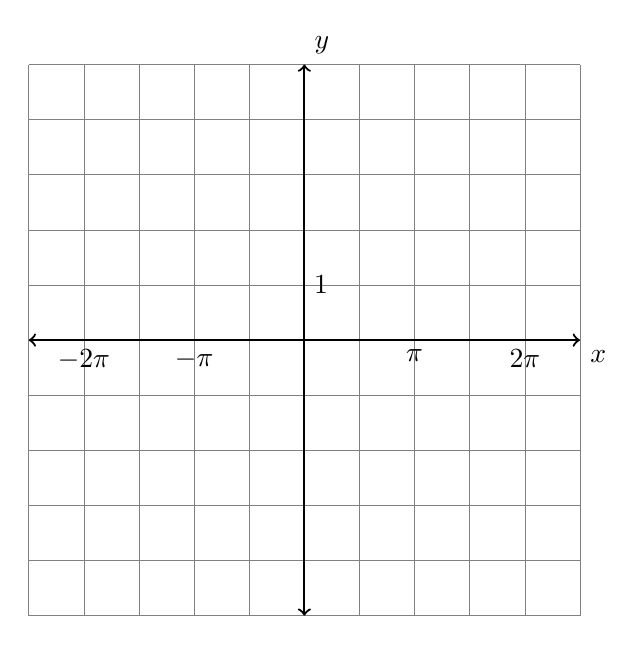
\begin{tikzpicture}[scale=0.7]
    \plane
    \end{tikzpicture}
\end{figure}
\question Sketch the graph of $-3\cos(x)-2.$
\begin{figure}[h]
\centering
    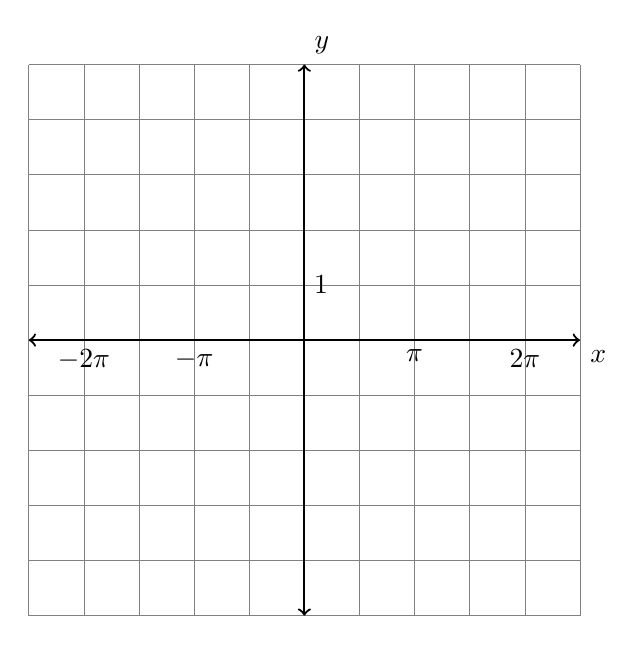
\begin{tikzpicture}[scale=0.7]
    \plane
    \end{tikzpicture}
\end{figure}
\newpage\subsection*{Quiz ID:319}
\question Using your calculator, find $\sin 1.6$
     \question Using your calculator find $\cos 143.65^{\circ}$
\question For an angle $\theta$ in quadrant I , if $ \tan\theta=\dfrac{3}{4}$ find $ \cos\theta $\makeemptybox{\stretch{1}}
\begin{table}[b]
\centering
\begin{tabular}{|l|l|l|l|l|l|l|}
\hline
\textbf{Question} & 1(/20) & 2(/20) & 3(/20) & 4(/20) & 5(/20) & \textbf{Total (/100)} \\ \hline
\textbf{Score}    &        &        &        &        &        &                      \\ \hline
\end{tabular}
\end{table}
\end{questions}\newpage
\section*{Quiz 45}
\subsection*{Quiz ID: 320}
\makebox[0.4\textwidth]{English Name:\enspace\hrulefill}
\vspace{0.5cm}\
\makebox[0.4\textwidth]{Chinese Name:\enspace\hrulefill}
\vspace{1cm}\
\begin{questions}
\question Sketch the graph of $4\sin(x)+1$.
\begin{figure}[h]
\centering
    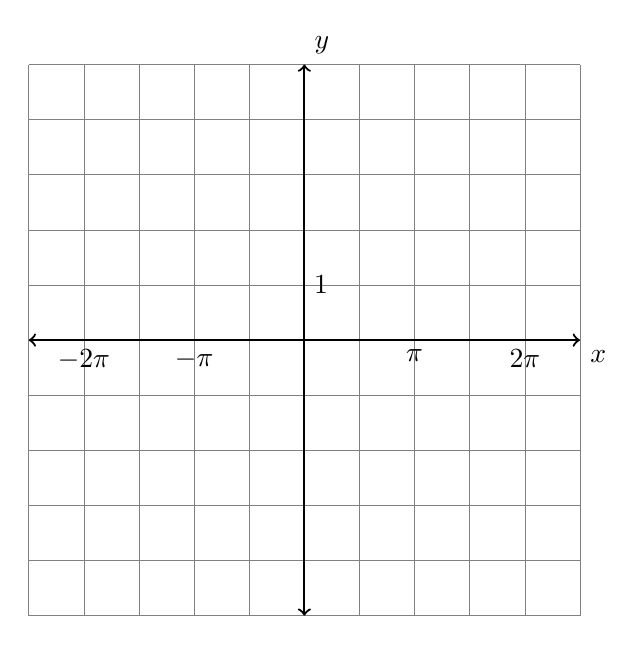
\begin{tikzpicture}[scale=0.7]
    \plane
    \end{tikzpicture}
\end{figure}
\question Sketch the graph of $-4\cos(x)-1.$
\begin{figure}[h]
\centering
    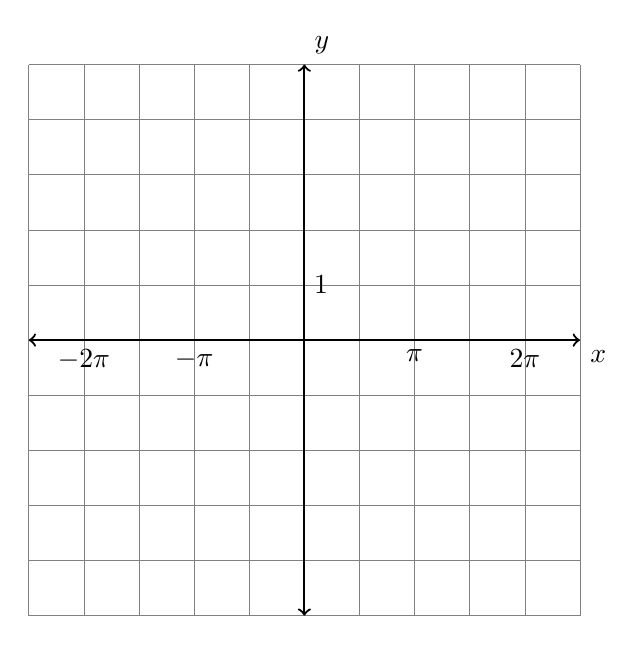
\begin{tikzpicture}[scale=0.7]
    \plane
    \end{tikzpicture}
\end{figure}
\newpage\subsection*{Quiz ID:320}
\question Using your calculator, find $\sin 1.95$
     \question Using your calculator find $\cos 87.25^{\circ}$
\question For an angle $\theta$ in quadrant I , if $ \cos\theta=\dfrac{6}{\sqrt{52}}$ find $ \cot\theta $\makeemptybox{\stretch{1}}
\begin{table}[b]
\centering
\begin{tabular}{|l|l|l|l|l|l|l|}
\hline
\textbf{Question} & 1(/20) & 2(/20) & 3(/20) & 4(/20) & 5(/20) & \textbf{Total (/100)} \\ \hline
\textbf{Score}    &        &        &        &        &        &                      \\ \hline
\end{tabular}
\end{table}
\end{questions}\newpage
\section*{Quiz 45}
\subsection*{Quiz ID: 321}
\makebox[0.4\textwidth]{English Name:\enspace\hrulefill}
\vspace{0.5cm}\
\makebox[0.4\textwidth]{Chinese Name:\enspace\hrulefill}
\vspace{1cm}\
\begin{questions}
\question Sketch the graph of $4\sin(x)+1$.
\begin{figure}[h]
\centering
    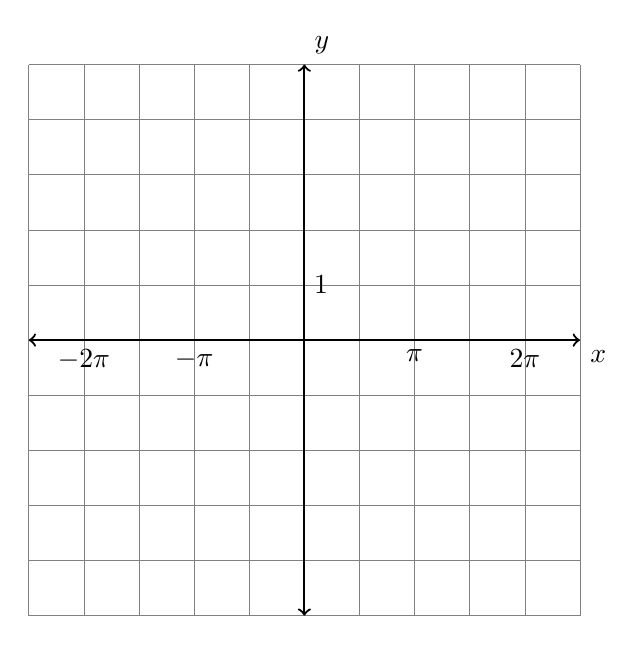
\begin{tikzpicture}[scale=0.7]
    \plane
    \end{tikzpicture}
\end{figure}
\question Sketch the graph of $-3\cos(x)-2.$
\begin{figure}[h]
\centering
    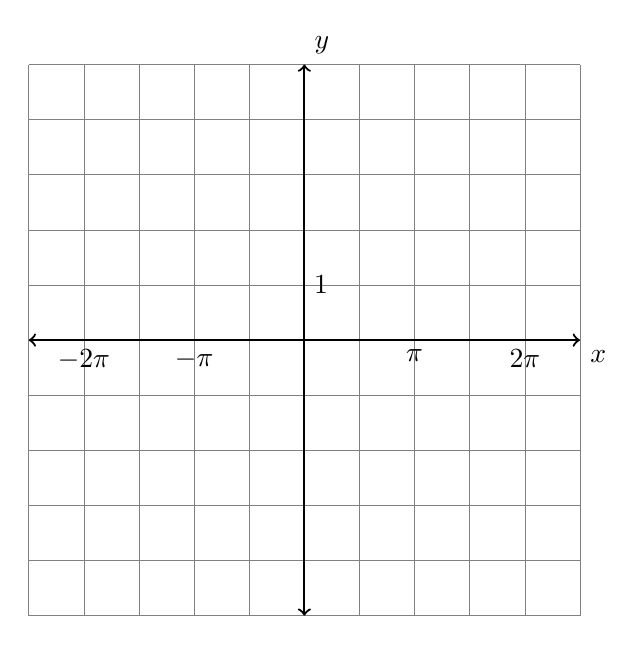
\begin{tikzpicture}[scale=0.7]
    \plane
    \end{tikzpicture}
\end{figure}
\newpage\subsection*{Quiz ID:321}
\question Using your calculator, find $\sin 2.65$
     \question Using your calculator find $\cos 9.7^{\circ}$
\question For an angle $\theta$ in quadrant I , if $ \cot\theta=\dfrac{6}{3}$ find $ \tan\theta $\makeemptybox{\stretch{1}}
\begin{table}[b]
\centering
\begin{tabular}{|l|l|l|l|l|l|l|}
\hline
\textbf{Question} & 1(/20) & 2(/20) & 3(/20) & 4(/20) & 5(/20) & \textbf{Total (/100)} \\ \hline
\textbf{Score}    &        &        &        &        &        &                      \\ \hline
\end{tabular}
\end{table}
\end{questions}\newpage
\section*{Quiz 45}
\subsection*{Quiz ID: 322}
\makebox[0.4\textwidth]{English Name:\enspace\hrulefill}
\vspace{0.5cm}\
\makebox[0.4\textwidth]{Chinese Name:\enspace\hrulefill}
\vspace{1cm}\
\begin{questions}
\question Sketch the graph of $2\sin(x)+1$.
\begin{figure}[h]
\centering
    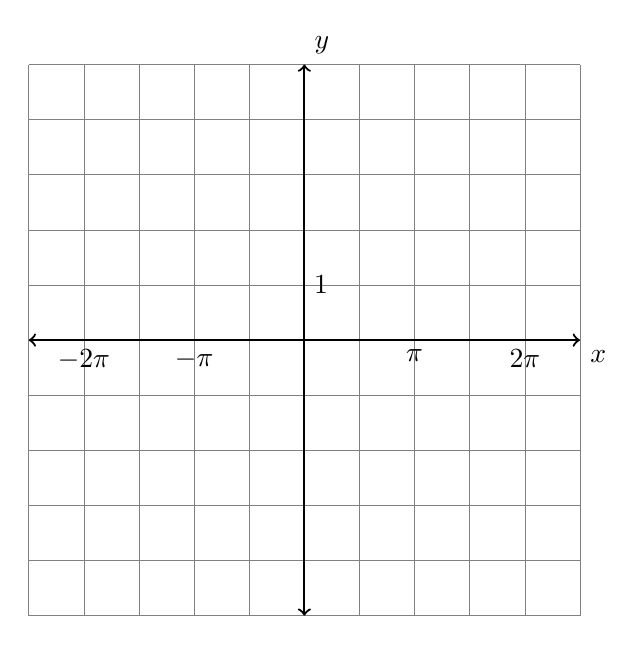
\begin{tikzpicture}[scale=0.7]
    \plane
    \end{tikzpicture}
\end{figure}
\question Sketch the graph of $-3\cos(x)-1.$
\begin{figure}[h]
\centering
    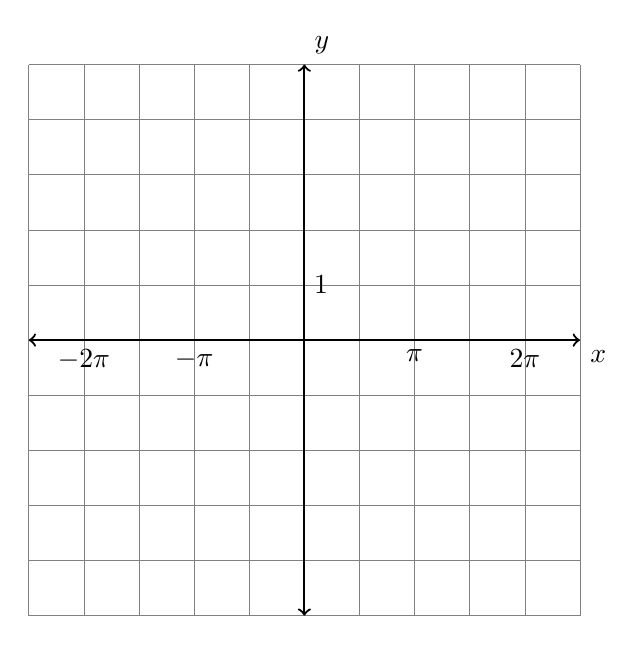
\begin{tikzpicture}[scale=0.7]
    \plane
    \end{tikzpicture}
\end{figure}
\newpage\subsection*{Quiz ID:322}
\question Using your calculator, find $\sin 3.35$
     \question Using your calculator find $\cos 75.5^{\circ}$
\question For an angle $\theta$ in quadrant I , if $ \sin\theta=\dfrac{4}{\sqrt{52}}$ find $ \sec\theta $\makeemptybox{\stretch{1}}
\begin{table}[b]
\centering
\begin{tabular}{|l|l|l|l|l|l|l|}
\hline
\textbf{Question} & 1(/20) & 2(/20) & 3(/20) & 4(/20) & 5(/20) & \textbf{Total (/100)} \\ \hline
\textbf{Score}    &        &        &        &        &        &                      \\ \hline
\end{tabular}
\end{table}
\end{questions}\newpage
\section*{Quiz 45}
\subsection*{Quiz ID: 323}
\makebox[0.4\textwidth]{English Name:\enspace\hrulefill}
\vspace{0.5cm}\
\makebox[0.4\textwidth]{Chinese Name:\enspace\hrulefill}
\vspace{1cm}\
\begin{questions}
\question Sketch the graph of $3\sin(x)+1$.
\begin{figure}[h]
\centering
    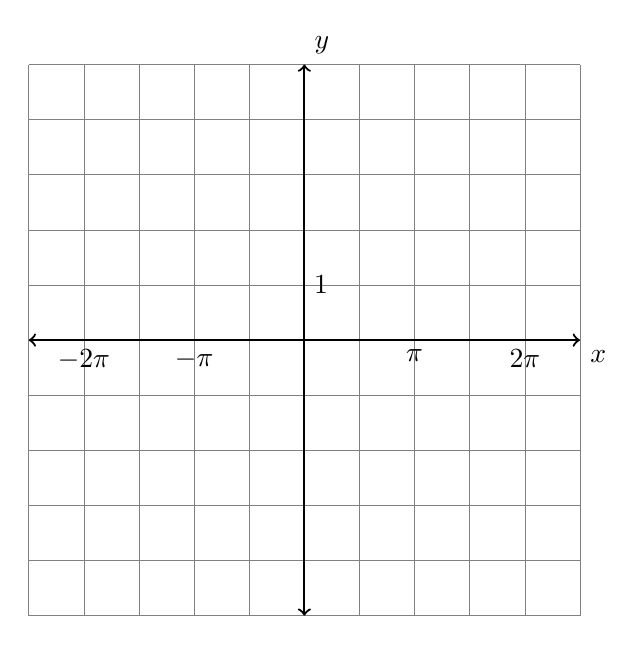
\begin{tikzpicture}[scale=0.7]
    \plane
    \end{tikzpicture}
\end{figure}
\question Sketch the graph of $-2\cos(x)-3.$
\begin{figure}[h]
\centering
    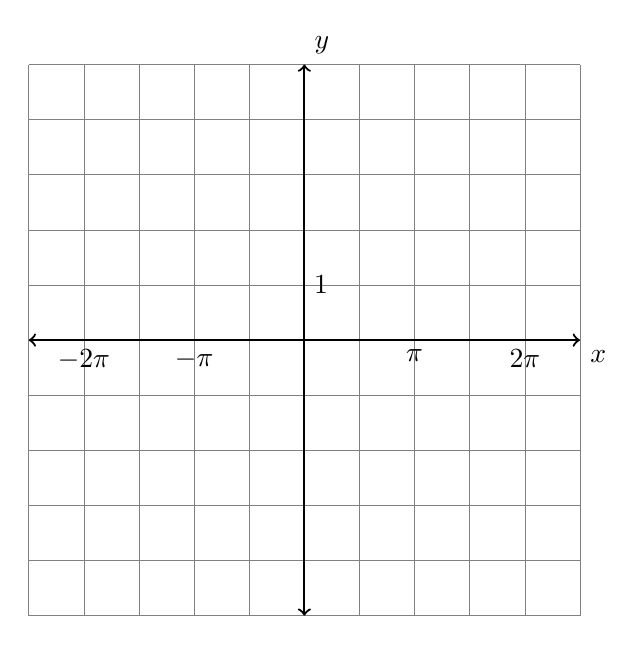
\begin{tikzpicture}[scale=0.7]
    \plane
    \end{tikzpicture}
\end{figure}
\newpage\subsection*{Quiz ID:323}
\question Using your calculator, find $\sin 1.25$
     \question Using your calculator find $\cos 146.0^{\circ}$
\question For an angle $\theta$ in quadrant I , if $ \cot\theta=\dfrac{5}{3}$ find $ \csc\theta $\makeemptybox{\stretch{1}}
\begin{table}[b]
\centering
\begin{tabular}{|l|l|l|l|l|l|l|}
\hline
\textbf{Question} & 1(/20) & 2(/20) & 3(/20) & 4(/20) & 5(/20) & \textbf{Total (/100)} \\ \hline
\textbf{Score}    &        &        &        &        &        &                      \\ \hline
\end{tabular}
\end{table}
\end{questions}\newpage
\section*{Quiz 45}
\subsection*{Quiz ID: 324}
\makebox[0.4\textwidth]{English Name:\enspace\hrulefill}
\vspace{0.5cm}\
\makebox[0.4\textwidth]{Chinese Name:\enspace\hrulefill}
\vspace{1cm}\
\begin{questions}
\question Sketch the graph of $2\sin(x)+2$.
\begin{figure}[h]
\centering
    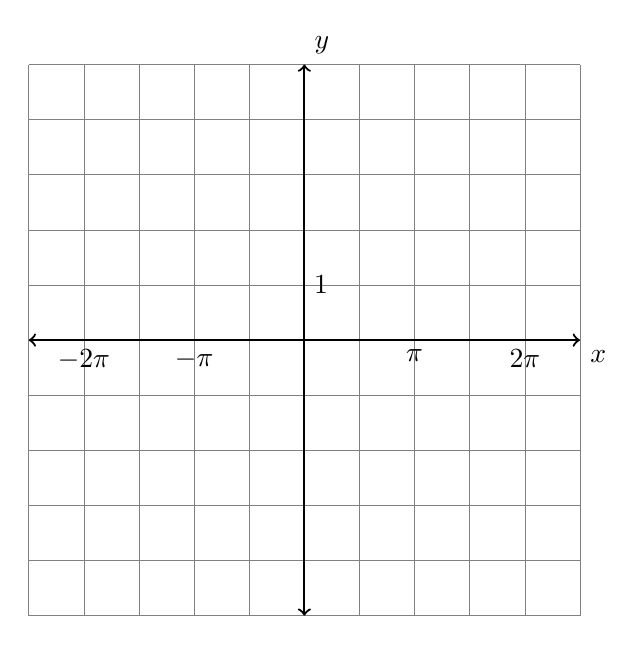
\begin{tikzpicture}[scale=0.7]
    \plane
    \end{tikzpicture}
\end{figure}
\question Sketch the graph of $-2\cos(x)-1.$
\begin{figure}[h]
\centering
    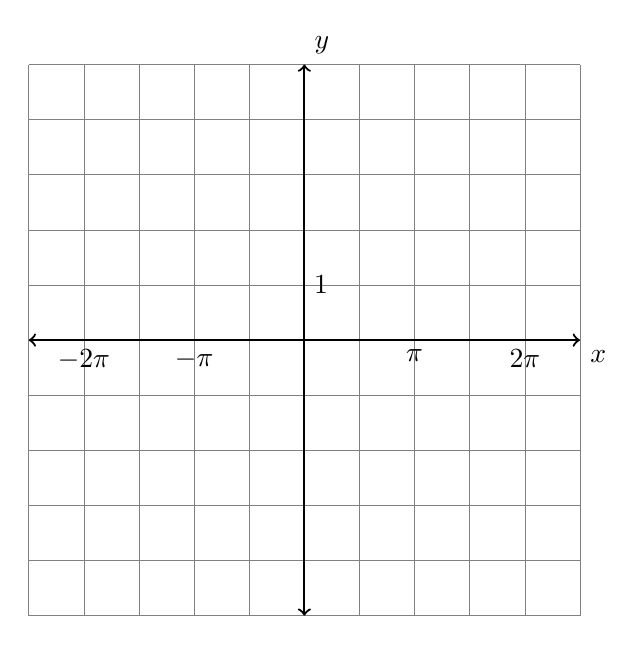
\begin{tikzpicture}[scale=0.7]
    \plane
    \end{tikzpicture}
\end{figure}
\newpage\subsection*{Quiz ID:324}
\question Using your calculator, find $\sin 5.45$
     \question Using your calculator find $\cos 141.3^{\circ}$
\question For an angle $\theta$ in quadrant I , if $ \sec\theta=\dfrac{5}{4}$ find $ \tan\theta $\makeemptybox{\stretch{1}}
\begin{table}[b]
\centering
\begin{tabular}{|l|l|l|l|l|l|l|}
\hline
\textbf{Question} & 1(/20) & 2(/20) & 3(/20) & 4(/20) & 5(/20) & \textbf{Total (/100)} \\ \hline
\textbf{Score}    &        &        &        &        &        &                      \\ \hline
\end{tabular}
\end{table}
\end{questions}\newpage
\section*{Quiz 45}
\subsection*{Quiz ID: 325}
\makebox[0.4\textwidth]{English Name:\enspace\hrulefill}
\vspace{0.5cm}\
\makebox[0.4\textwidth]{Chinese Name:\enspace\hrulefill}
\vspace{1cm}\
\begin{questions}
\question Sketch the graph of $4\sin(x)+1$.
\begin{figure}[h]
\centering
    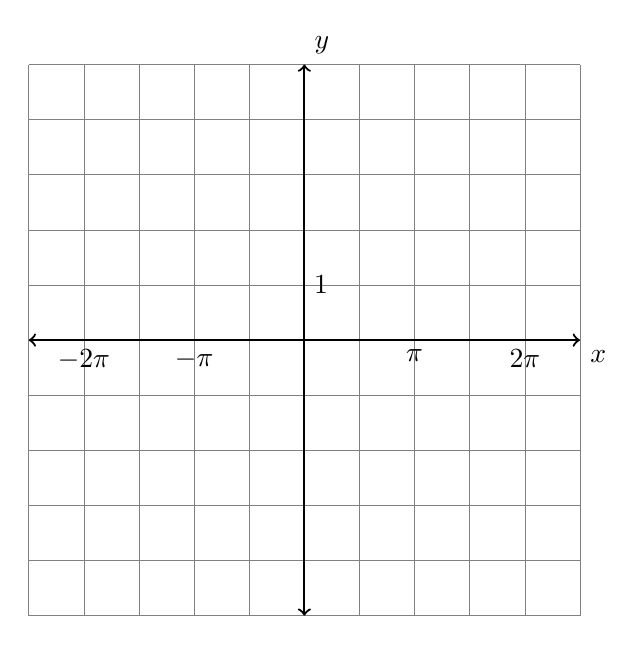
\begin{tikzpicture}[scale=0.7]
    \plane
    \end{tikzpicture}
\end{figure}
\question Sketch the graph of $-3\cos(x)-1.$
\begin{figure}[h]
\centering
    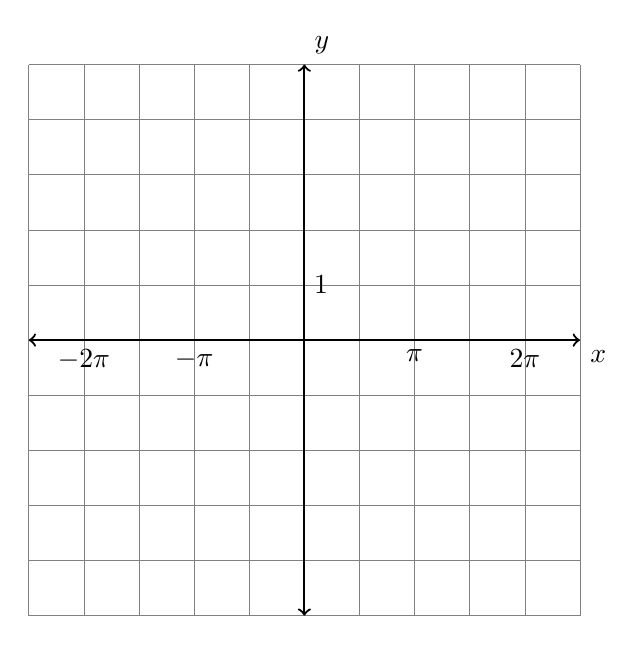
\begin{tikzpicture}[scale=0.7]
    \plane
    \end{tikzpicture}
\end{figure}
\newpage\subsection*{Quiz ID:325}
\question Using your calculator, find $\sin 4.75$
     \question Using your calculator find $\cos 14.4^{\circ}$
\question For an angle $\theta$ in quadrant I , if $ \sin\theta=\dfrac{4}{\sqrt{52}}$ find $ \csc\theta $\makeemptybox{\stretch{1}}
\begin{table}[b]
\centering
\begin{tabular}{|l|l|l|l|l|l|l|}
\hline
\textbf{Question} & 1(/20) & 2(/20) & 3(/20) & 4(/20) & 5(/20) & \textbf{Total (/100)} \\ \hline
\textbf{Score}    &        &        &        &        &        &                      \\ \hline
\end{tabular}
\end{table}
\end{questions}\newpage
\section*{Quiz 45}
\subsection*{Quiz ID: 326}
\makebox[0.4\textwidth]{English Name:\enspace\hrulefill}
\vspace{0.5cm}\
\makebox[0.4\textwidth]{Chinese Name:\enspace\hrulefill}
\vspace{1cm}\
\begin{questions}
\question Sketch the graph of $4\sin(x)+1$.
\begin{figure}[h]
\centering
    \begin{tikzpicture}[scale=0.7]
    \plane
    \end{tikzpicture}
\end{figure}
\question Sketch the graph of $-2\cos(x)-3.$
\begin{figure}[h]
\centering
    \begin{tikzpicture}[scale=0.7]
    \plane
    \end{tikzpicture}
\end{figure}
\newpage\subsection*{Quiz ID:326}
\question Using your calculator, find $\sin 4.05$
     \question Using your calculator find $\cos 77.85^{\circ}$
\question For an angle $\theta$ in quadrant I , if $ \sin\theta=\dfrac{3}{5}$ find $ \cot\theta $\makeemptybox{\stretch{1}}
\begin{table}[b]
\centering
\begin{tabular}{|l|l|l|l|l|l|l|}
\hline
\textbf{Question} & 1(/20) & 2(/20) & 3(/20) & 4(/20) & 5(/20) & \textbf{Total (/100)} \\ \hline
\textbf{Score}    &        &        &        &        &        &                      \\ \hline
\end{tabular}
\end{table}
\end{questions}\newpage
\section*{Quiz 45}
\subsection*{Quiz ID: 327}
\makebox[0.4\textwidth]{English Name:\enspace\hrulefill}
\vspace{0.5cm}\
\makebox[0.4\textwidth]{Chinese Name:\enspace\hrulefill}
\vspace{1cm}\
\begin{questions}
\question Sketch the graph of $4\sin(x)+1$.
\begin{figure}[h]
\centering
    \begin{tikzpicture}[scale=0.7]
    \plane
    \end{tikzpicture}
\end{figure}
\question Sketch the graph of $-3\cos(x)-2.$
\begin{figure}[h]
\centering
    \begin{tikzpicture}[scale=0.7]
    \plane
    \end{tikzpicture}
\end{figure}
\newpage\subsection*{Quiz ID:327}
\question Using your calculator, find $\sin 2.65$
     \question Using your calculator find $\cos 176.55^{\circ}$
\question For an angle $\theta$ in quadrant I , if $ \tan\theta=\dfrac{3}{4}$ find $ \sin\theta $\makeemptybox{\stretch{1}}
\begin{table}[b]
\centering
\begin{tabular}{|l|l|l|l|l|l|l|}
\hline
\textbf{Question} & 1(/20) & 2(/20) & 3(/20) & 4(/20) & 5(/20) & \textbf{Total (/100)} \\ \hline
\textbf{Score}    &        &        &        &        &        &                      \\ \hline
\end{tabular}
\end{table}
\end{questions}\newpage
\section*{Quiz 45}
\subsection*{Quiz ID: 328}
\makebox[0.4\textwidth]{English Name:\enspace\hrulefill}
\vspace{0.5cm}\
\makebox[0.4\textwidth]{Chinese Name:\enspace\hrulefill}
\vspace{1cm}\
\begin{questions}
\question Sketch the graph of $2\sin(x)+2$.
\begin{figure}[h]
\centering
    \begin{tikzpicture}[scale=0.7]
    \plane
    \end{tikzpicture}
\end{figure}
\question Sketch the graph of $-3\cos(x)-2.$
\begin{figure}[h]
\centering
    \begin{tikzpicture}[scale=0.7]
    \plane
    \end{tikzpicture}
\end{figure}
\newpage\subsection*{Quiz ID:328}
\question Using your calculator, find $\sin 2.65$
     \question Using your calculator find $\cos 157.75^{\circ}$
\question For an angle $\theta$ in quadrant I , if $ \tan\theta=\dfrac{2}{4}$ find $ \sin\theta $\makeemptybox{\stretch{1}}
\begin{table}[b]
\centering
\begin{tabular}{|l|l|l|l|l|l|l|}
\hline
\textbf{Question} & 1(/20) & 2(/20) & 3(/20) & 4(/20) & 5(/20) & \textbf{Total (/100)} \\ \hline
\textbf{Score}    &        &        &        &        &        &                      \\ \hline
\end{tabular}
\end{table}
\end{questions}\newpage
\section*{Quiz 45}
\subsection*{Quiz ID: 329}
\makebox[0.4\textwidth]{English Name:\enspace\hrulefill}
\vspace{0.5cm}\
\makebox[0.4\textwidth]{Chinese Name:\enspace\hrulefill}
\vspace{1cm}\
\begin{questions}
\question Sketch the graph of $2\sin(x)+3$.
\begin{figure}[h]
\centering
    \begin{tikzpicture}[scale=0.7]
    \plane
    \end{tikzpicture}
\end{figure}
\question Sketch the graph of $-4\cos(x)-1.$
\begin{figure}[h]
\centering
    \begin{tikzpicture}[scale=0.7]
    \plane
    \end{tikzpicture}
\end{figure}
\newpage\subsection*{Quiz ID:329}
\question Using your calculator, find $\sin 0.55$
     \question Using your calculator find $\cos 127.2^{\circ}$
\question For an angle $\theta$ in quadrant I , if $ \csc\theta=\dfrac{\sqrt{20}}{2}$ find $ \tan\theta $\makeemptybox{\stretch{1}}
\begin{table}[b]
\centering
\begin{tabular}{|l|l|l|l|l|l|l|}
\hline
\textbf{Question} & 1(/20) & 2(/20) & 3(/20) & 4(/20) & 5(/20) & \textbf{Total (/100)} \\ \hline
\textbf{Score}    &        &        &        &        &        &                      \\ \hline
\end{tabular}
\end{table}
\end{questions}\newpage
\section*{Quiz 45}
\subsection*{Quiz ID: 330}
\makebox[0.4\textwidth]{English Name:\enspace\hrulefill}
\vspace{0.5cm}\
\makebox[0.4\textwidth]{Chinese Name:\enspace\hrulefill}
\vspace{1cm}\
\begin{questions}
\question Sketch the graph of $4\sin(x)+1$.
\begin{figure}[h]
\centering
    \begin{tikzpicture}[scale=0.7]
    \plane
    \end{tikzpicture}
\end{figure}
\question Sketch the graph of $-3\cos(x)-1.$
\begin{figure}[h]
\centering
    \begin{tikzpicture}[scale=0.7]
    \plane
    \end{tikzpicture}
\end{figure}
\newpage\subsection*{Quiz ID:330}
\question Using your calculator, find $\sin 5.45$
     \question Using your calculator find $\cos 28.5^{\circ}$
\question For an angle $\theta$ in quadrant I , if $ \sin\theta=\dfrac{2}{\sqrt{20}}$ find $ \cos\theta $\makeemptybox{\stretch{1}}
\begin{table}[b]
\centering
\begin{tabular}{|l|l|l|l|l|l|l|}
\hline
\textbf{Question} & 1(/20) & 2(/20) & 3(/20) & 4(/20) & 5(/20) & \textbf{Total (/100)} \\ \hline
\textbf{Score}    &        &        &        &        &        &                      \\ \hline
\end{tabular}
\end{table}
\end{questions}\newpage
\section*{Quiz 45}
\subsection*{Quiz ID: 331}
\makebox[0.4\textwidth]{English Name:\enspace\hrulefill}
\vspace{0.5cm}\
\makebox[0.4\textwidth]{Chinese Name:\enspace\hrulefill}
\vspace{1cm}\
\begin{questions}
\question Sketch the graph of $2\sin(x)+1$.
\begin{figure}[h]
\centering
    \begin{tikzpicture}[scale=0.7]
    \plane
    \end{tikzpicture}
\end{figure}
\question Sketch the graph of $-2\cos(x)-3.$
\begin{figure}[h]
\centering
    \begin{tikzpicture}[scale=0.7]
    \plane
    \end{tikzpicture}
\end{figure}
\newpage\subsection*{Quiz ID:331}
\question Using your calculator, find $\sin 5.45$
     \question Using your calculator find $\cos 134.25^{\circ}$
\question For an angle $\theta$ in quadrant I , if $ \sec\theta=\dfrac{\sqrt{45}}{6}$ find $ \tan\theta $\makeemptybox{\stretch{1}}
\begin{table}[b]
\centering
\begin{tabular}{|l|l|l|l|l|l|l|}
\hline
\textbf{Question} & 1(/20) & 2(/20) & 3(/20) & 4(/20) & 5(/20) & \textbf{Total (/100)} \\ \hline
\textbf{Score}    &        &        &        &        &        &                      \\ \hline
\end{tabular}
\end{table}
\end{questions}\newpage
\section*{Quiz 45}
\subsection*{Quiz ID: 332}
\makebox[0.4\textwidth]{English Name:\enspace\hrulefill}
\vspace{0.5cm}\
\makebox[0.4\textwidth]{Chinese Name:\enspace\hrulefill}
\vspace{1cm}\
\begin{questions}
\question Sketch the graph of $2\sin(x)+1$.
\begin{figure}[h]
\centering
    \begin{tikzpicture}[scale=0.7]
    \plane
    \end{tikzpicture}
\end{figure}
\question Sketch the graph of $-3\cos(x)-2.$
\begin{figure}[h]
\centering
    \begin{tikzpicture}[scale=0.7]
    \plane
    \end{tikzpicture}
\end{figure}
\newpage\subsection*{Quiz ID:332}
\question Using your calculator, find $\sin 1.25$
     \question Using your calculator find $\cos 49.65^{\circ}$
\question For an angle $\theta$ in quadrant I , if $ \cot\theta=\dfrac{5}{4}$ find $ \csc\theta $\makeemptybox{\stretch{1}}
\begin{table}[b]
\centering
\begin{tabular}{|l|l|l|l|l|l|l|}
\hline
\textbf{Question} & 1(/20) & 2(/20) & 3(/20) & 4(/20) & 5(/20) & \textbf{Total (/100)} \\ \hline
\textbf{Score}    &        &        &        &        &        &                      \\ \hline
\end{tabular}
\end{table}
\end{questions}\newpage
\section*{Quiz 45}
\subsection*{Quiz ID: 333}
\makebox[0.4\textwidth]{English Name:\enspace\hrulefill}
\vspace{0.5cm}\
\makebox[0.4\textwidth]{Chinese Name:\enspace\hrulefill}
\vspace{1cm}\
\begin{questions}
\question Sketch the graph of $2\sin(x)+2$.
\begin{figure}[h]
\centering
    \begin{tikzpicture}[scale=0.7]
    \plane
    \end{tikzpicture}
\end{figure}
\question Sketch the graph of $-2\cos(x)-2.$
\begin{figure}[h]
\centering
    \begin{tikzpicture}[scale=0.7]
    \plane
    \end{tikzpicture}
\end{figure}
\newpage\subsection*{Quiz ID:333}
\question Using your calculator, find $\sin 1.6$
     \question Using your calculator find $\cos 113.1^{\circ}$
\question For an angle $\theta$ in quadrant I , if $ \tan\theta=\dfrac{2}{6}$ find $ \sec\theta $\makeemptybox{\stretch{1}}
\begin{table}[b]
\centering
\begin{tabular}{|l|l|l|l|l|l|l|}
\hline
\textbf{Question} & 1(/20) & 2(/20) & 3(/20) & 4(/20) & 5(/20) & \textbf{Total (/100)} \\ \hline
\textbf{Score}    &        &        &        &        &        &                      \\ \hline
\end{tabular}
\end{table}
\end{questions}\newpage
\section*{Quiz 45}
\subsection*{Quiz ID: 334}
\makebox[0.4\textwidth]{English Name:\enspace\hrulefill}
\vspace{0.5cm}\
\makebox[0.4\textwidth]{Chinese Name:\enspace\hrulefill}
\vspace{1cm}\
\begin{questions}
\question Sketch the graph of $3\sin(x)+2$.
\begin{figure}[h]
\centering
    \begin{tikzpicture}[scale=0.7]
    \plane
    \end{tikzpicture}
\end{figure}
\question Sketch the graph of $-2\cos(x)-3.$
\begin{figure}[h]
\centering
    \begin{tikzpicture}[scale=0.7]
    \plane
    \end{tikzpicture}
\end{figure}
\newpage\subsection*{Quiz ID:334}
\question Using your calculator, find $\sin 3.35$
     \question Using your calculator find $\cos 44.95^{\circ}$
\question For an angle $\theta$ in quadrant I , if $ \csc\theta=\dfrac{\sqrt{41}}{4}$ find $ \sin\theta $\makeemptybox{\stretch{1}}
\begin{table}[b]
\centering
\begin{tabular}{|l|l|l|l|l|l|l|}
\hline
\textbf{Question} & 1(/20) & 2(/20) & 3(/20) & 4(/20) & 5(/20) & \textbf{Total (/100)} \\ \hline
\textbf{Score}    &        &        &        &        &        &                      \\ \hline
\end{tabular}
\end{table}
\end{questions}\newpage
\section*{Quiz 45}
\subsection*{Quiz ID: 335}
\makebox[0.4\textwidth]{English Name:\enspace\hrulefill}
\vspace{0.5cm}\
\makebox[0.4\textwidth]{Chinese Name:\enspace\hrulefill}
\vspace{1cm}\
\begin{questions}
\question Sketch the graph of $2\sin(x)+3$.
\begin{figure}[h]
\centering
    \begin{tikzpicture}[scale=0.7]
    \plane
    \end{tikzpicture}
\end{figure}
\question Sketch the graph of $-2\cos(x)-2.$
\begin{figure}[h]
\centering
    \begin{tikzpicture}[scale=0.7]
    \plane
    \end{tikzpicture}
\end{figure}
\newpage\subsection*{Quiz ID:335}
\question Using your calculator, find $\sin 0.2$
     \question Using your calculator find $\cos 66.1^{\circ}$
\question For an angle $\theta$ in quadrant I , if $ \cos\theta=\dfrac{6}{\sqrt{40}}$ find $ \sin\theta $\makeemptybox{\stretch{1}}
\begin{table}[b]
\centering
\begin{tabular}{|l|l|l|l|l|l|l|}
\hline
\textbf{Question} & 1(/20) & 2(/20) & 3(/20) & 4(/20) & 5(/20) & \textbf{Total (/100)} \\ \hline
\textbf{Score}    &        &        &        &        &        &                      \\ \hline
\end{tabular}
\end{table}
\end{questions}\newpage
\section*{Quiz 45}
\subsection*{Quiz ID: 336}
\makebox[0.4\textwidth]{English Name:\enspace\hrulefill}
\vspace{0.5cm}\
\makebox[0.4\textwidth]{Chinese Name:\enspace\hrulefill}
\vspace{1cm}\
\begin{questions}
\question Sketch the graph of $4\sin(x)+1$.
\begin{figure}[h]
\centering
    \begin{tikzpicture}[scale=0.7]
    \plane
    \end{tikzpicture}
\end{figure}
\question Sketch the graph of $-3\cos(x)-1.$
\begin{figure}[h]
\centering
    \begin{tikzpicture}[scale=0.7]
    \plane
    \end{tikzpicture}
\end{figure}
\newpage\subsection*{Quiz ID:336}
\question Using your calculator, find $\sin 4.75$
     \question Using your calculator find $\cos 49.65^{\circ}$
\question For an angle $\theta$ in quadrant I , if $ \tan\theta=\dfrac{4}{6}$ find $ \cot\theta $\makeemptybox{\stretch{1}}
\begin{table}[b]
\centering
\begin{tabular}{|l|l|l|l|l|l|l|}
\hline
\textbf{Question} & 1(/20) & 2(/20) & 3(/20) & 4(/20) & 5(/20) & \textbf{Total (/100)} \\ \hline
\textbf{Score}    &        &        &        &        &        &                      \\ \hline
\end{tabular}
\end{table}
\end{questions}\newpage
\section*{Quiz 45}
\subsection*{Quiz ID: 337}
\makebox[0.4\textwidth]{English Name:\enspace\hrulefill}
\vspace{0.5cm}\
\makebox[0.4\textwidth]{Chinese Name:\enspace\hrulefill}
\vspace{1cm}\
\begin{questions}
\question Sketch the graph of $3\sin(x)+1$.
\begin{figure}[h]
\centering
    \begin{tikzpicture}[scale=0.7]
    \plane
    \end{tikzpicture}
\end{figure}
\question Sketch the graph of $-2\cos(x)-1.$
\begin{figure}[h]
\centering
    \begin{tikzpicture}[scale=0.7]
    \plane
    \end{tikzpicture}
\end{figure}
\newpage\subsection*{Quiz ID:337}
\question Using your calculator, find $\sin 0.2$
     \question Using your calculator find $\cos 54.35^{\circ}$
\question For an angle $\theta$ in quadrant I , if $ \sin\theta=\dfrac{4}{\sqrt{41}}$ find $ \cos\theta $\makeemptybox{\stretch{1}}
\begin{table}[b]
\centering
\begin{tabular}{|l|l|l|l|l|l|l|}
\hline
\textbf{Question} & 1(/20) & 2(/20) & 3(/20) & 4(/20) & 5(/20) & \textbf{Total (/100)} \\ \hline
\textbf{Score}    &        &        &        &        &        &                      \\ \hline
\end{tabular}
\end{table}
\end{questions}\newpage
\section*{Quiz 45}
\subsection*{Quiz ID: 338}
\makebox[0.4\textwidth]{English Name:\enspace\hrulefill}
\vspace{0.5cm}\
\makebox[0.4\textwidth]{Chinese Name:\enspace\hrulefill}
\vspace{1cm}\
\begin{questions}
\question Sketch the graph of $3\sin(x)+1$.
\begin{figure}[h]
\centering
    \begin{tikzpicture}[scale=0.7]
    \plane
    \end{tikzpicture}
\end{figure}
\question Sketch the graph of $-4\cos(x)-1.$
\begin{figure}[h]
\centering
    \begin{tikzpicture}[scale=0.7]
    \plane
    \end{tikzpicture}
\end{figure}
\newpage\subsection*{Quiz ID:338}
\question Using your calculator, find $\sin 4.75$
     \question Using your calculator find $\cos 131.9^{\circ}$
\question For an angle $\theta$ in quadrant I , if $ \cot\theta=\dfrac{5}{3}$ find $ \csc\theta $\makeemptybox{\stretch{1}}
\begin{table}[b]
\centering
\begin{tabular}{|l|l|l|l|l|l|l|}
\hline
\textbf{Question} & 1(/20) & 2(/20) & 3(/20) & 4(/20) & 5(/20) & \textbf{Total (/100)} \\ \hline
\textbf{Score}    &        &        &        &        &        &                      \\ \hline
\end{tabular}
\end{table}
\end{questions}\newpage
\section*{Quiz 45}
\subsection*{Quiz ID: 339}
\makebox[0.4\textwidth]{English Name:\enspace\hrulefill}
\vspace{0.5cm}\
\makebox[0.4\textwidth]{Chinese Name:\enspace\hrulefill}
\vspace{1cm}\
\begin{questions}
\question Sketch the graph of $2\sin(x)+2$.
\begin{figure}[h]
\centering
    \begin{tikzpicture}[scale=0.7]
    \plane
    \end{tikzpicture}
\end{figure}
\question Sketch the graph of $-2\cos(x)-2.$
\begin{figure}[h]
\centering
    \begin{tikzpicture}[scale=0.7]
    \plane
    \end{tikzpicture}
\end{figure}
\newpage\subsection*{Quiz ID:339}
\question Using your calculator, find $\sin 0.2$
     \question Using your calculator find $\cos 108.4^{\circ}$
\question For an angle $\theta$ in quadrant I , if $ \tan\theta=\dfrac{3}{6}$ find $ \cos\theta $\makeemptybox{\stretch{1}}
\begin{table}[b]
\centering
\begin{tabular}{|l|l|l|l|l|l|l|}
\hline
\textbf{Question} & 1(/20) & 2(/20) & 3(/20) & 4(/20) & 5(/20) & \textbf{Total (/100)} \\ \hline
\textbf{Score}    &        &        &        &        &        &                      \\ \hline
\end{tabular}
\end{table}
\end{questions}\newpage
\section*{Quiz 45}
\subsection*{Quiz ID: 340}
\makebox[0.4\textwidth]{English Name:\enspace\hrulefill}
\vspace{0.5cm}\
\makebox[0.4\textwidth]{Chinese Name:\enspace\hrulefill}
\vspace{1cm}\
\begin{questions}
\question Sketch the graph of $2\sin(x)+2$.
\begin{figure}[h]
\centering
    \begin{tikzpicture}[scale=0.7]
    \plane
    \end{tikzpicture}
\end{figure}
\question Sketch the graph of $-4\cos(x)-1.$
\begin{figure}[h]
\centering
    \begin{tikzpicture}[scale=0.7]
    \plane
    \end{tikzpicture}
\end{figure}
\newpage\subsection*{Quiz ID:340}
\question Using your calculator, find $\sin 3.0$
     \question Using your calculator find $\cos 150.7^{\circ}$
\question For an angle $\theta$ in quadrant I , if $ \csc\theta=\dfrac{5}{3}$ find $ \cot\theta $\makeemptybox{\stretch{1}}
\begin{table}[b]
\centering
\begin{tabular}{|l|l|l|l|l|l|l|}
\hline
\textbf{Question} & 1(/20) & 2(/20) & 3(/20) & 4(/20) & 5(/20) & \textbf{Total (/100)} \\ \hline
\textbf{Score}    &        &        &        &        &        &                      \\ \hline
\end{tabular}
\end{table}
\end{questions}\newpage
\section*{Quiz 45}
\subsection*{Quiz ID: 341}
\makebox[0.4\textwidth]{English Name:\enspace\hrulefill}
\vspace{0.5cm}\
\makebox[0.4\textwidth]{Chinese Name:\enspace\hrulefill}
\vspace{1cm}\
\begin{questions}
\question Sketch the graph of $3\sin(x)+1$.
\begin{figure}[h]
\centering
    \begin{tikzpicture}[scale=0.7]
    \plane
    \end{tikzpicture}
\end{figure}
\question Sketch the graph of $-3\cos(x)-1.$
\begin{figure}[h]
\centering
    \begin{tikzpicture}[scale=0.7]
    \plane
    \end{tikzpicture}
\end{figure}
\newpage\subsection*{Quiz ID:341}
\question Using your calculator, find $\sin 1.25$
     \question Using your calculator find $\cos 96.65^{\circ}$
\question For an angle $\theta$ in quadrant I , if $ \sin\theta=\dfrac{4}{\sqrt{41}}$ find $ \sec\theta $\makeemptybox{\stretch{1}}
\begin{table}[b]
\centering
\begin{tabular}{|l|l|l|l|l|l|l|}
\hline
\textbf{Question} & 1(/20) & 2(/20) & 3(/20) & 4(/20) & 5(/20) & \textbf{Total (/100)} \\ \hline
\textbf{Score}    &        &        &        &        &        &                      \\ \hline
\end{tabular}
\end{table}
\end{questions}\newpage
\section*{Quiz 45}
\subsection*{Quiz ID: 342}
\makebox[0.4\textwidth]{English Name:\enspace\hrulefill}
\vspace{0.5cm}\
\makebox[0.4\textwidth]{Chinese Name:\enspace\hrulefill}
\vspace{1cm}\
\begin{questions}
\question Sketch the graph of $4\sin(x)+1$.
\begin{figure}[h]
\centering
    \begin{tikzpicture}[scale=0.7]
    \plane
    \end{tikzpicture}
\end{figure}
\question Sketch the graph of $-3\cos(x)-1.$
\begin{figure}[h]
\centering
    \begin{tikzpicture}[scale=0.7]
    \plane
    \end{tikzpicture}
\end{figure}
\newpage\subsection*{Quiz ID:342}
\question Using your calculator, find $\sin 5.45$
     \question Using your calculator find $\cos 120.15^{\circ}$
\question For an angle $\theta$ in quadrant I , if $ \cos\theta=\dfrac{4}{5}$ find $ \sin\theta $\makeemptybox{\stretch{1}}
\begin{table}[b]
\centering
\begin{tabular}{|l|l|l|l|l|l|l|}
\hline
\textbf{Question} & 1(/20) & 2(/20) & 3(/20) & 4(/20) & 5(/20) & \textbf{Total (/100)} \\ \hline
\textbf{Score}    &        &        &        &        &        &                      \\ \hline
\end{tabular}
\end{table}
\end{questions}\newpage
\section*{Quiz 45}
\subsection*{Quiz ID: 343}
\makebox[0.4\textwidth]{English Name:\enspace\hrulefill}
\vspace{0.5cm}\
\makebox[0.4\textwidth]{Chinese Name:\enspace\hrulefill}
\vspace{1cm}\
\begin{questions}
\question Sketch the graph of $3\sin(x)+1$.
\begin{figure}[h]
\centering
    \begin{tikzpicture}[scale=0.7]
    \plane
    \end{tikzpicture}
\end{figure}
\question Sketch the graph of $-4\cos(x)-1.$
\begin{figure}[h]
\centering
    \begin{tikzpicture}[scale=0.7]
    \plane
    \end{tikzpicture}
\end{figure}
\newpage\subsection*{Quiz ID:343}
\question Using your calculator, find $\sin 0.55$
     \question Using your calculator find $\cos 75.5^{\circ}$
\question For an angle $\theta$ in quadrant I , if $ \cot\theta=\dfrac{5}{2}$ find $ \csc\theta $\makeemptybox{\stretch{1}}
\begin{table}[b]
\centering
\begin{tabular}{|l|l|l|l|l|l|l|}
\hline
\textbf{Question} & 1(/20) & 2(/20) & 3(/20) & 4(/20) & 5(/20) & \textbf{Total (/100)} \\ \hline
\textbf{Score}    &        &        &        &        &        &                      \\ \hline
\end{tabular}
\end{table}
\end{questions}\newpage
\section*{Quiz 45}
\subsection*{Quiz ID: 344}
\makebox[0.4\textwidth]{English Name:\enspace\hrulefill}
\vspace{0.5cm}\
\makebox[0.4\textwidth]{Chinese Name:\enspace\hrulefill}
\vspace{1cm}\
\begin{questions}
\question Sketch the graph of $2\sin(x)+1$.
\begin{figure}[h]
\centering
    \begin{tikzpicture}[scale=0.7]
    \plane
    \end{tikzpicture}
\end{figure}
\question Sketch the graph of $-3\cos(x)-1.$
\begin{figure}[h]
\centering
    \begin{tikzpicture}[scale=0.7]
    \plane
    \end{tikzpicture}
\end{figure}
\newpage\subsection*{Quiz ID:344}
\question Using your calculator, find $\sin 5.1$
     \question Using your calculator find $\cos 70.8^{\circ}$
\question For an angle $\theta$ in quadrant I , if $ \sin\theta=\dfrac{5}{\sqrt{61}}$ find $ \cos\theta $\makeemptybox{\stretch{1}}
\begin{table}[b]
\centering
\begin{tabular}{|l|l|l|l|l|l|l|}
\hline
\textbf{Question} & 1(/20) & 2(/20) & 3(/20) & 4(/20) & 5(/20) & \textbf{Total (/100)} \\ \hline
\textbf{Score}    &        &        &        &        &        &                      \\ \hline
\end{tabular}
\end{table}
\end{questions}\newpage
\section*{Quiz 45}
\subsection*{Quiz ID: 345}
\makebox[0.4\textwidth]{English Name:\enspace\hrulefill}
\vspace{0.5cm}\
\makebox[0.4\textwidth]{Chinese Name:\enspace\hrulefill}
\vspace{1cm}\
\begin{questions}
\question Sketch the graph of $4\sin(x)+1$.
\begin{figure}[h]
\centering
    \begin{tikzpicture}[scale=0.7]
    \plane
    \end{tikzpicture}
\end{figure}
\question Sketch the graph of $-4\cos(x)-1.$
\begin{figure}[h]
\centering
    \begin{tikzpicture}[scale=0.7]
    \plane
    \end{tikzpicture}
\end{figure}
\newpage\subsection*{Quiz ID:345}
\question Using your calculator, find $\sin 5.8$
     \question Using your calculator find $\cos 127.2^{\circ}$
\question For an angle $\theta$ in quadrant I , if $ \sec\theta=\dfrac{\sqrt{40}}{6}$ find $ \tan\theta $\makeemptybox{\stretch{1}}
\begin{table}[b]
\centering
\begin{tabular}{|l|l|l|l|l|l|l|}
\hline
\textbf{Question} & 1(/20) & 2(/20) & 3(/20) & 4(/20) & 5(/20) & \textbf{Total (/100)} \\ \hline
\textbf{Score}    &        &        &        &        &        &                      \\ \hline
\end{tabular}
\end{table}
\end{questions}\newpage
\section*{Quiz 45}
\subsection*{Quiz ID: 346}
\makebox[0.4\textwidth]{English Name:\enspace\hrulefill}
\vspace{0.5cm}\
\makebox[0.4\textwidth]{Chinese Name:\enspace\hrulefill}
\vspace{1cm}\
\begin{questions}
\question Sketch the graph of $3\sin(x)+1$.
\begin{figure}[h]
\centering
    \begin{tikzpicture}[scale=0.7]
    \plane
    \end{tikzpicture}
\end{figure}
\question Sketch the graph of $-2\cos(x)-2.$
\begin{figure}[h]
\centering
    \begin{tikzpicture}[scale=0.7]
    \plane
    \end{tikzpicture}
\end{figure}
\newpage\subsection*{Quiz ID:346}
\question Using your calculator, find $\sin 2.65$
     \question Using your calculator find $\cos 103.7^{\circ}$
\question For an angle $\theta$ in quadrant I , if $ \tan\theta=\dfrac{3}{5}$ find $ \csc\theta $\makeemptybox{\stretch{1}}
\begin{table}[b]
\centering
\begin{tabular}{|l|l|l|l|l|l|l|}
\hline
\textbf{Question} & 1(/20) & 2(/20) & 3(/20) & 4(/20) & 5(/20) & \textbf{Total (/100)} \\ \hline
\textbf{Score}    &        &        &        &        &        &                      \\ \hline
\end{tabular}
\end{table}
\end{questions}\newpage
\section*{Quiz 45}
\subsection*{Quiz ID: 347}
\makebox[0.4\textwidth]{English Name:\enspace\hrulefill}
\vspace{0.5cm}\
\makebox[0.4\textwidth]{Chinese Name:\enspace\hrulefill}
\vspace{1cm}\
\begin{questions}
\question Sketch the graph of $3\sin(x)+1$.
\begin{figure}[h]
\centering
    \begin{tikzpicture}[scale=0.7]
    \plane
    \end{tikzpicture}
\end{figure}
\question Sketch the graph of $-2\cos(x)-1.$
\begin{figure}[h]
\centering
    \begin{tikzpicture}[scale=0.7]
    \plane
    \end{tikzpicture}
\end{figure}
\newpage\subsection*{Quiz ID:347}
\question Using your calculator, find $\sin 5.8$
     \question Using your calculator find $\cos 23.8^{\circ}$
\question For an angle $\theta$ in quadrant I , if $ \tan\theta=\dfrac{2}{5}$ find $ \sin\theta $\makeemptybox{\stretch{1}}
\begin{table}[b]
\centering
\begin{tabular}{|l|l|l|l|l|l|l|}
\hline
\textbf{Question} & 1(/20) & 2(/20) & 3(/20) & 4(/20) & 5(/20) & \textbf{Total (/100)} \\ \hline
\textbf{Score}    &        &        &        &        &        &                      \\ \hline
\end{tabular}
\end{table}
\end{questions}\newpage
\section*{Quiz 45}
\subsection*{Quiz ID: 348}
\makebox[0.4\textwidth]{English Name:\enspace\hrulefill}
\vspace{0.5cm}\
\makebox[0.4\textwidth]{Chinese Name:\enspace\hrulefill}
\vspace{1cm}\
\begin{questions}
\question Sketch the graph of $4\sin(x)+1$.
\begin{figure}[h]
\centering
    \begin{tikzpicture}[scale=0.7]
    \plane
    \end{tikzpicture}
\end{figure}
\question Sketch the graph of $-4\cos(x)-1.$
\begin{figure}[h]
\centering
    \begin{tikzpicture}[scale=0.7]
    \plane
    \end{tikzpicture}
\end{figure}
\newpage\subsection*{Quiz ID:348}
\question Using your calculator, find $\sin 4.4$
     \question Using your calculator find $\cos 171.85^{\circ}$
\question For an angle $\theta$ in quadrant I , if $ \cos\theta=\dfrac{4}{5}$ find $ \csc\theta $\makeemptybox{\stretch{1}}
\begin{table}[b]
\centering
\begin{tabular}{|l|l|l|l|l|l|l|}
\hline
\textbf{Question} & 1(/20) & 2(/20) & 3(/20) & 4(/20) & 5(/20) & \textbf{Total (/100)} \\ \hline
\textbf{Score}    &        &        &        &        &        &                      \\ \hline
\end{tabular}
\end{table}
\end{questions}\newpage
\section*{Quiz 45}
\subsection*{Quiz ID: 349}
\makebox[0.4\textwidth]{English Name:\enspace\hrulefill}
\vspace{0.5cm}\
\makebox[0.4\textwidth]{Chinese Name:\enspace\hrulefill}
\vspace{1cm}\
\begin{questions}
\question Sketch the graph of $3\sin(x)+2$.
\begin{figure}[h]
\centering
    \begin{tikzpicture}[scale=0.7]
    \plane
    \end{tikzpicture}
\end{figure}
\question Sketch the graph of $-3\cos(x)-1.$
\begin{figure}[h]
\centering
    \begin{tikzpicture}[scale=0.7]
    \plane
    \end{tikzpicture}
\end{figure}
\newpage\subsection*{Quiz ID:349}
\question Using your calculator, find $\sin 4.05$
     \question Using your calculator find $\cos 33.2^{\circ}$
\question For an angle $\theta$ in quadrant I , if $ \cos\theta=\dfrac{6}{\sqrt{45}}$ find $ \tan\theta $\makeemptybox{\stretch{1}}
\begin{table}[b]
\centering
\begin{tabular}{|l|l|l|l|l|l|l|}
\hline
\textbf{Question} & 1(/20) & 2(/20) & 3(/20) & 4(/20) & 5(/20) & \textbf{Total (/100)} \\ \hline
\textbf{Score}    &        &        &        &        &        &                      \\ \hline
\end{tabular}
\end{table}
\end{questions}\newpage
\section*{Quiz 45}
\subsection*{Quiz ID: 350}
\makebox[0.4\textwidth]{English Name:\enspace\hrulefill}
\vspace{0.5cm}\
\makebox[0.4\textwidth]{Chinese Name:\enspace\hrulefill}
\vspace{1cm}\
\begin{questions}
\question Sketch the graph of $2\sin(x)+3$.
\begin{figure}[h]
\centering
    \begin{tikzpicture}[scale=0.7]
    \plane
    \end{tikzpicture}
\end{figure}
\question Sketch the graph of $-4\cos(x)-1.$
\begin{figure}[h]
\centering
    \begin{tikzpicture}[scale=0.7]
    \plane
    \end{tikzpicture}
\end{figure}
\newpage\subsection*{Quiz ID:350}
\question Using your calculator, find $\sin 4.75$
     \question Using your calculator find $\cos 9.7^{\circ}$
\question For an angle $\theta$ in quadrant I , if $ \cos\theta=\dfrac{6}{\sqrt{40}}$ find $ \tan\theta $\makeemptybox{\stretch{1}}
\begin{table}[b]
\centering
\begin{tabular}{|l|l|l|l|l|l|l|}
\hline
\textbf{Question} & 1(/20) & 2(/20) & 3(/20) & 4(/20) & 5(/20) & \textbf{Total (/100)} \\ \hline
\textbf{Score}    &        &        &        &        &        &                      \\ \hline
\end{tabular}
\end{table}
\end{questions}\newpage
\section*{Quiz 45}
\subsection*{Quiz ID: 351}
\makebox[0.4\textwidth]{English Name:\enspace\hrulefill}
\vspace{0.5cm}\
\makebox[0.4\textwidth]{Chinese Name:\enspace\hrulefill}
\vspace{1cm}\
\begin{questions}
\question Sketch the graph of $3\sin(x)+2$.
\begin{figure}[h]
\centering
    \begin{tikzpicture}[scale=0.7]
    \plane
    \end{tikzpicture}
\end{figure}
\question Sketch the graph of $-4\cos(x)-1.$
\begin{figure}[h]
\centering
    \begin{tikzpicture}[scale=0.7]
    \plane
    \end{tikzpicture}
\end{figure}
\newpage\subsection*{Quiz ID:351}
\question Using your calculator, find $\sin 1.95$
     \question Using your calculator find $\cos 70.8^{\circ}$
\question For an angle $\theta$ in quadrant I , if $ \cot\theta=\dfrac{3}{2}$ find $ \csc\theta $\makeemptybox{\stretch{1}}
\begin{table}[b]
\centering
\begin{tabular}{|l|l|l|l|l|l|l|}
\hline
\textbf{Question} & 1(/20) & 2(/20) & 3(/20) & 4(/20) & 5(/20) & \textbf{Total (/100)} \\ \hline
\textbf{Score}    &        &        &        &        &        &                      \\ \hline
\end{tabular}
\end{table}
\end{questions}\newpage
\section*{Quiz 45}
\subsection*{Quiz ID: 352}
\makebox[0.4\textwidth]{English Name:\enspace\hrulefill}
\vspace{0.5cm}\
\makebox[0.4\textwidth]{Chinese Name:\enspace\hrulefill}
\vspace{1cm}\
\begin{questions}
\question Sketch the graph of $2\sin(x)+2$.
\begin{figure}[h]
\centering
    \begin{tikzpicture}[scale=0.7]
    \plane
    \end{tikzpicture}
\end{figure}
\question Sketch the graph of $-2\cos(x)-2.$
\begin{figure}[h]
\centering
    \begin{tikzpicture}[scale=0.7]
    \plane
    \end{tikzpicture}
\end{figure}
\newpage\subsection*{Quiz ID:352}
\question Using your calculator, find $\sin 0.2$
     \question Using your calculator find $\cos 28.5^{\circ}$
\question For an angle $\theta$ in quadrant I , if $ \sec\theta=\dfrac{\sqrt{45}}{6}$ find $ \tan\theta $\makeemptybox{\stretch{1}}
\begin{table}[b]
\centering
\begin{tabular}{|l|l|l|l|l|l|l|}
\hline
\textbf{Question} & 1(/20) & 2(/20) & 3(/20) & 4(/20) & 5(/20) & \textbf{Total (/100)} \\ \hline
\textbf{Score}    &        &        &        &        &        &                      \\ \hline
\end{tabular}
\end{table}
\end{questions}\newpage
\section*{Quiz 45}
\subsection*{Quiz ID: 353}
\makebox[0.4\textwidth]{English Name:\enspace\hrulefill}
\vspace{0.5cm}\
\makebox[0.4\textwidth]{Chinese Name:\enspace\hrulefill}
\vspace{1cm}\
\begin{questions}
\question Sketch the graph of $2\sin(x)+1$.
\begin{figure}[h]
\centering
    \begin{tikzpicture}[scale=0.7]
    \plane
    \end{tikzpicture}
\end{figure}
\question Sketch the graph of $-3\cos(x)-1.$
\begin{figure}[h]
\centering
    \begin{tikzpicture}[scale=0.7]
    \plane
    \end{tikzpicture}
\end{figure}
\newpage\subsection*{Quiz ID:353}
\question Using your calculator, find $\sin 3.0$
     \question Using your calculator find $\cos 143.65^{\circ}$
\question For an angle $\theta$ in quadrant I , if $ \cos\theta=\dfrac{4}{5}$ find $ \cot\theta $\makeemptybox{\stretch{1}}
\begin{table}[b]
\centering
\begin{tabular}{|l|l|l|l|l|l|l|}
\hline
\textbf{Question} & 1(/20) & 2(/20) & 3(/20) & 4(/20) & 5(/20) & \textbf{Total (/100)} \\ \hline
\textbf{Score}    &        &        &        &        &        &                      \\ \hline
\end{tabular}
\end{table}
\end{questions}\newpage
\section*{Quiz 45}
\subsection*{Quiz ID: 354}
\makebox[0.4\textwidth]{English Name:\enspace\hrulefill}
\vspace{0.5cm}\
\makebox[0.4\textwidth]{Chinese Name:\enspace\hrulefill}
\vspace{1cm}\
\begin{questions}
\question Sketch the graph of $3\sin(x)+2$.
\begin{figure}[h]
\centering
    \begin{tikzpicture}[scale=0.7]
    \plane
    \end{tikzpicture}
\end{figure}
\question Sketch the graph of $-4\cos(x)-1.$
\begin{figure}[h]
\centering
    \begin{tikzpicture}[scale=0.7]
    \plane
    \end{tikzpicture}
\end{figure}
\newpage\subsection*{Quiz ID:354}
\question Using your calculator, find $\sin 4.4$
     \question Using your calculator find $\cos 33.2^{\circ}$
\question For an angle $\theta$ in quadrant I , if $ \cot\theta=\dfrac{5}{2}$ find $ \cos\theta $\makeemptybox{\stretch{1}}
\begin{table}[b]
\centering
\begin{tabular}{|l|l|l|l|l|l|l|}
\hline
\textbf{Question} & 1(/20) & 2(/20) & 3(/20) & 4(/20) & 5(/20) & \textbf{Total (/100)} \\ \hline
\textbf{Score}    &        &        &        &        &        &                      \\ \hline
\end{tabular}
\end{table}
\end{questions}\newpage
\section*{Quiz 45}
\subsection*{Quiz ID: 355}
\makebox[0.4\textwidth]{English Name:\enspace\hrulefill}
\vspace{0.5cm}\
\makebox[0.4\textwidth]{Chinese Name:\enspace\hrulefill}
\vspace{1cm}\
\begin{questions}
\question Sketch the graph of $4\sin(x)+1$.
\begin{figure}[h]
\centering
    \begin{tikzpicture}[scale=0.7]
    \plane
    \end{tikzpicture}
\end{figure}
\question Sketch the graph of $-2\cos(x)-3.$
\begin{figure}[h]
\centering
    \begin{tikzpicture}[scale=0.7]
    \plane
    \end{tikzpicture}
\end{figure}
\newpage\subsection*{Quiz ID:355}
\question Using your calculator, find $\sin 1.6$
     \question Using your calculator find $\cos 68.45^{\circ}$
\question For an angle $\theta$ in quadrant I , if $ \sin\theta=\dfrac{5}{\sqrt{61}}$ find $ \cot\theta $\makeemptybox{\stretch{1}}
\begin{table}[b]
\centering
\begin{tabular}{|l|l|l|l|l|l|l|}
\hline
\textbf{Question} & 1(/20) & 2(/20) & 3(/20) & 4(/20) & 5(/20) & \textbf{Total (/100)} \\ \hline
\textbf{Score}    &        &        &        &        &        &                      \\ \hline
\end{tabular}
\end{table}
\end{questions}\newpage
\end{document}
